\documentclass[conference]{IEEEtran}
\IEEEoverridecommandlockouts
% The preceding line is only needed to identify funding in the first footnote. If that is unneeded, please comment it out.
\usepackage{multirow,makecell}
\usepackage{cite}
\usepackage{amsmath,amssymb,amsfonts}
\usepackage{algorithmic}
\usepackage{graphicx}
\usepackage{textcomp}
\usepackage{xcolor}
\def\BibTeX{{\rm B\kern-.05em{\sc i\kern-.025em b}\kern-.08em
    T\kern-.1667em\lower.7ex\hbox{E}\kern-.125emX}}
\begin{document}

\title{Pesonalized AssemblyMminutes Information Providing Service \\
}
\author{\IEEEauthorblockN{Sangwon Kim}
\IEEEauthorblockA{\textit{dept. information system} \\
\textit{Hanyang University}\\
Seoul, Korea  \\
tkddnjs2014@gmail.com}
\and
\IEEEauthorblockN{Kyumin Kim }
\IEEEauthorblockA{\textit{dept. information system} \\
\textit{Hanyang University}\\
Seoul, Korea \\
kkyumin@gmail.com}
\and
\IEEEauthorblockN{Injun Hwang}
\IEEEauthorblockA{\textit{dept. information system} \\
\textit{Hanyang University}\\
Seoul, Korea \\
 sroo2315@gmail.com}
\and
\IEEEauthorblockN{Hyunho Kim}
\IEEEauthorblockA{\textit{dept. information system} \\
\textit{Hanyang University}\\
Seoul, Korea \\
jwalag87@gmail.com}
}
\maketitle

\begin{abstract}
The purpose of our service is to help the general public access easily to assembly minutes. The public will be provided not only minutes but also looking up minutes per agenda, participated politician, and his statements, interested keywords. Through this service, the public can judge politician on real statement, not edited information of media.\linebreak \\
\end{abstract}

\begin{IEEEkeywords}
Politics, Speech, Keyword Analysis, Minutes of Government Meetings, AI Speaker  \linebreak \\
\end{IEEEkeywords}

  \begin{table}[htbp]
  \renewcommand{\arraystretch}{1.7}
\caption{Role Assignments}
\begin{center}
\begin{tabular}{|p{1.5cm}|p{1.8cm}|p{4.2cm}|}
\hline
\textbf{Roles} & \textbf{{Name}}& \textbf{{Task description and etc.}} \\
\hline
User & NUGU speaker users & The user’s needs are the final goal of the project. They want to make their lives easier and more efficient through the output of the project. They can raise concerns and necessities to the project if their needs don’t meet up to satisfaction. It is the most important their rules in a project.  \\
\hline
Customer & SKT & Customers demand to the project to make satisfied with users. Customers are located between Develop teams and users. The user’s needs through the whole project are really close to the main purpose of their rules because they are closely related to their interests. They want project teams to use NUGU speaker to satisfy users.  \\
\hline
Software \linebreak Developers& Hyunho Kim \linebreak Kyumin Kim& Software developers are main resources of the the project. Their technical stacks and engineering skills create actual product. They demand core function requirements to Development managers which give them up to their developing process. Their final goal is to satisfy users and customers by realizing close to the requirements. \\
\hline
\end{tabular}
\label{tab1}
\end{center}
\end{table}

  \begin{table}[htbp]
  \renewcommand{\arraystretch}{1.7}
\begin{center}
\begin{tabular}{|p{1.5cm}|p{1.8cm}|p{4.2cm}|}
\hline
\textbf{Roles} & \textbf{{Name}}& \textbf{{Task description and etc.}} \\
\hline

Development \linebreak managers& Sangwon Kim \linebreak Injun Hwang& Development mangers intercommunicate with Customer and Software developer to satisfy with whole stakeholders. They schedule timelines to stick to the project before deadline. They build overall developing design process. So they should figure out what they are confronted by, such as threats and variables, plan projects and direct business matters that Software developers can’t handle with. They support Software developers to focus on developing processes. \\
\hline
\end{tabular}
\label{tab1}
\end{center}
\end{table}

\vspace{5mm}

\section{Introduction}
In Korea, there’s a fashioned sentence “The general publics are dog and pig”. This sentence was just a script of Korean movie, “Insiders”, but it gives sympathies to many citizens. Our team started to think about why this sentence is caught in the minds of the people.

The articles of Korean presses tend to be writed on suggestive, prejudiced by inclination of that press rather than political facts, while editing politician’s opinions or moves. Also, the presses tend to report only in just portion of facts, only in favor of certain political orientations. Consequently the public can’t decide whether that article is neutral or biased on amicable organizations. So they tend to be instigated by that biased report quite often unknowing the facts. In fact, when looking at Naver(the largest portal site of Korea)’s political news article, a lot of people are instigated, unilaterally and aggressively commenting on the contents due to stimulating titles or contents that mixed with specific utterances and reporters' opinions. So Naver often hides highest recommended in such articles.

It means there is a lack of fact information that politic can’t judge politician objectively. Current articles are processed based on reporter’s political orientation, so people are more and more complicated, and can’t make decide based on their criteria. To escape on this situation, some people make an effort to access on assembly site to judge that certain politician’s utterances and their political orientation. But, finding information only on facts is not just easy. It brings about three problems below.

First, the most objective way to determine what a politician has spoken is to hear and judge pure speech of politician, not someone else’s refined words. Usually, the politician speaks something that is full of political beliefs in the political meeting. It would be a fact information that politic can determine about the politician. The public fact data of the politician in the internet are just only on election records, award records, criminal facts, etc. These simple examples don’t provide inclination of the politician. Hence, our team got conviction that the real opinion of politician is in the congressional records. Therefore, our team will develop a service that can verify what politician has spoken by serving  assembly minutes easily.

Second, the way to find congressional records is too complex. Congressional records in the assembly are typed by stenographer, and opened to the public through National Assembly Minutes. Public should link in National Assembly Minutes System and download pdf files to find remarks. Many citizens don’t interested in politics because it doesn’t give any monetary benefits or it doesn’t give fun to them. To turn their minds, minimized way to get information of politicians is needed. The National Assembly Minutes that doesn’t provide convenience to the citizen is just a nominal system. So our team decide to give information about Assembly minutes to citizen easily through web page. Also, we would like to use AI speaker to fulfill desires of various people.

Furthermore, the current minutes is not classified of its contents and politicians. The file name of minutes just designates on conference date and order. If the user wants to find specific agenda, they need to search it manually by scrolling the pdf files. So our team decide to give solution of this problem. We are going to parse all of the minutes and after classify the politician’s agenda and speech in the minutes. Also, we will make keyword searching system. This service will provide an useful function that search specific agenda and politician to users. It will be applied to AI speaker to make our service more useful.

The AI speaker(Smart speaker) is a kind of wireless speaker, which is activated by more than one impressive words(hot words). Voice-Command-Device wh ch embed The Virtual Assistant carries out co-interactive functions and hands-free commands.

The biggest difference between AI Speaker and typical Speaker is that the AI speaker recognizes “Speech Recognition” to perform specific commands like listening to music, setting alarm and timer, searching information like News, weather, etc. The main input and output unit of Speech-Recognition device is built-in Microphone and Speaker. The AI speaker is consisted of such like these simple units, so it is efficient to send and receive information than any other smartphone, smart TV.

Accordingly, the biggest advantage of using AI speaker is to order AI something by “Speak some words” when the user is doing some other things on their own hands or can’t type some words through smart device. For example, when the user is on the verge of falling asleep or busy for ready to go out, the user can’t afford to use a smart device. In addition, the old age people cannot afford to read long texts like minutes. So service is suitable for this people.

Specifically, The NUGU speaker is the first Korean-made AI speaker made by SKT in 2016. Over the last two years, The NUGU speaker so far developed a lot so typical functions such as mentioned above are already applied. So our team had to decide to make service that speaker doesn’t provide and groundbreaking service

Third, There is no current services that gather personalized inclined politician or his related field. By lacking of information of politicians, just some specific politicians are reminded to citizens. Though, even if the politician is not popular, some people’s area of interest can be similar to him. Maybe they want to subscribe regularly of that politician.When they want to find information of him, but they will find out that there are only refined, edited version of his mentions. So, based on whole minutes of specific politician’s participated, we will make a interested aria or keyword extraction service through big data analysis. This will be a good method to listen on politician who is similar to user’s interested area by setting up user’s keyword of interested area and scrapping of his activation.

In conclusion, we want to make a  personalized subscribe system of interested politician so the politic can determine of the politician based on objective facts. For this, our team will make service that meet four functions. first, recognizing specific politician’s statements by looking up assembly minutes. second, printing the words through web service and AI speaker. third, the function that finding agenda or politician easily. fourth, a method to listen on politician who is similar to user’s interested area by setting up user’s keyword of interested area and scrapping of his activation. Through this service, It is anticipated that the public’s independence and judgement will be improved.


\section{Requirements}
\subsection{Public}
The public can be provided with  not only providing information on the minutes of the assembly but also detailed functions of the minutes. They can be provided by inquiring about the minutes of the parliamentary minutes, inquiring agendas involving politicians, inquiring of politicians speech, and inquiring of politicians' keywords of interest.\\ 

\begin{enumerate}
	\item \textit {Log-in Page:} 
In the log-in page, the user can saves specific politicians or interested keywords individually. subscribed politician, interested keywords are saved in backend server. through this, the user can uses subscribe or registering functions.\\
    \begin{enumerate}
    	\item \textit {Log-in:} Log-in page is a first page that users can see when they enter to our website. These functions will log in a user based on a username and password being matched in a database.\\
        \item \textit {ID/PW search:} This page is for users who forgot their ID or PW.\\
    \end{enumerate}
    
    \item \textit {Main Page:}  The main page is a key feature of this service. Users can search for detailed information about minutes. To concrete this, the following functions are implemented. \\
    \begin{enumerate}
    	\item \textit {Looking up function about meeting contents per agenda :} Users can view agendas by organizing meeting files by agenda\\
        \item \textit {Looking up function about agenda participating specific politicians :} Users can search agenda in which a specific politician participates.\\
        \item \textit {Looking up  function about politician’s' speech according to agenda :} Users can inquire politician’s' speech according to agenda\\
        \item \textit {Looking up function of politics’ interested keyword :} users can inquire about politics’ interested keyword\\
        \item \textit {subscribing function about concerned politics :} users can subscribe about concerned politics.\
        \item \textit {ILooking up  function about subscribing politics :} Users can inquire about subscribing politics’ speech\\
        \item \textit {registering of concerned politics keyword :} Users can be recommended about politics by using concerened keyword
        \\
        \\
        \\
        \\
        \\
        \\
        \\
        \\
        \\
        \\
        \\
        \\
        \\
        \\
        \\
        \\
        \\
        \\
    \end{enumerate}
\end{enumerate}
\section{Related Works}
We have researched for softwares that are doing similar works or having similar logics to ours. There are some tools that are providing similar service with different logics, in different platform about politic software. By doing this research, we found out that software about politics is widely used in various kinds of fields and it has a lot of potential powers. 

\subsection{g0v}
  \begin{figure}[htbp]
	\centerline{
\includegraphics[width=89mm, scale=0.5]{fig/g0v.png}}
	\caption{g0v}
	\label{fig}
	\end{figure}
The g0v is an open source, open government collaboration started by Chia-liang Kao, ipa, kirby and others in late 2012 in Taiwan. Originally driven by a bimonthly hackathon, the community has expanded to include different professional and non-information technology background members. a "forked" version of that agency with contributions by civic hackers. Continuing this inspiration from the software development world, the forked content can then be "merged" back into the government agency's website. g0v is a community that promotes the transparency of government information and is committed to developing information platforms and tools for citizens to participate in society. As of the beginning of 2014, there have been contributors across three continents, and the results have been released in a free software model that embraces knowledge sharing.
\\
\\

\subsection{Gov track}
  \begin{figure}[htbp]
	\centerline{
\includegraphics[width=89mm, scale=0.5]{fig/gov_track.jpg}}
	\caption{Gov track}
	\label{fig}
	\end{figure}
	
GovTrack.us is a website developed by then-student Joshua Tauberer. It is based in Washington, D.C., and was launched as a hobby. It enables its users to track the bills and members of the United States Congress. Users can add trackers to certain bills, thereby narrowing the scope of the information they receive. The website collects data on members of Congress, allowing users to check members' voting records and attendance relative to their peers. It propagates the ideology of increasing transparency in the government and building better communication between the general public and the government.
\\
\\
\\
\\
\\

\subsection{sunlight foundation}
  \begin{figure}[htbp]
	\centerline{
\includegraphics[width=89mm, scale=0.5]{fig/sunlight_foundation.png}}
	\caption{sunlight foundation}
	\label{fig}
	\end{figure}
The Sunlight Foundation is an American 501 nonpartisan, nonprofit organization that advocates for open government. The organization was founded in April 2006 with the goal of increasing transparency and accountability in the United States Congress, the executive branch, and in state and local governments. The foundation's primary focus is the role of money in politics. The organization seeks to increase campaign finance regulations and disclosure requirements.The Sunlight Foundation advocates for more regulation and limitations regarding campaign finance. The organization opposed the ruling in Citizens United v. FEC, calling it "disastrous.". The organization supported the DISCLOSE Act, a congressional bill that would have enacted stricter campaign finance regulations by requiring increased disclosure of political spending in federal elections. The Sunlight Foundation believes that Congress should mandate real-time online disclosure of political contributions. It opposes dark money, or funds given to nonprofit organizations that are not required to disclose their donors.
\\
\\
\\
\\
\\
\\
\\
\\

\subsection{Brigade media}
  \begin{figure}[htbp]
	\centerline{
\includegraphics[width=89mm, scale=0.5]{fig/brigade_media.jpg}}
	\caption{Brigade media}
	\label{fig}
	\end{figure}
Brigade Media, also known as Brigade, is a civic technology platform that was formed on June 4, 2014, and founded by James Windon, Jason Putorti, John Thrall, Matt Mahan, and Miche Capone. The platform is intended to serve as a way for users to connect with others who share the same or similar views and voice their opinions, create debates, or organize petitions. This process is intended to make the users' concerns more visible to and influential towards United States' policymakers. One mission of Brigade Media is to act as a foreground for its users to connect and organize so that they can voice their opinions on our nation's issues. Another more general goal is to increase voter participation. Brigade interacts with American voters by linking its users to the same held concerns. The opinions of elected officials on those concerns will be provided and metrics about the candidate most similar in concerns and degree of concern will be available. This data should be useful for both candidates and voters, in that voters can voice their grievances and candidates must respond accordingly.

\section{Development Environment}
\subsection{Choice of development platform}
\begin{enumerate}
  \item 
  \textit{Used platform and why}
	
We will going to use Linux OS platform, specifically Ubuntu ver 16.04 LTS.  (Ubuntu is free, completely customizable, resource-friendly than Windows platform.) Furthermore, Linux command line is the biggest reason to use this platform. Its Bash(Shell) with a various command makes our development process easy.
In addition, our team going to use Amazon Web Service(AWS) to upload our service to cloud server. Amazon Elastic Compute Cloud (EC2) is a leading infrastructure cloud service that offers scalable compute capacity in the cloud. It allows clients to rent powerful virtual computers and run their own applications. To use this, we have to boot an Amazon Machine Image(AMI). AMI Ubuntu ver 16.04 LTS is provided by the AWS in free tier, so we decide to use. Continuity with local OS version with server OS version helps to develop without problems that occur due to OS differences.
\\
  
   \item \textit{Used Programming Language and why}
       \begin{enumerate}
    	\item \textit{Python 3.7}
\\The Python Package Index(PyPI) contains numerous third-party modules that make Python capable of interacting with most of the other languages and platforms. Python provides a large standard library which includes areas like internet protocols, string operations, web services tools and operating system interfaces. Many high use programming tasks have already been scripted into the standard library which reduces length of code to be written significantly.\\

        \item \textit{Java 1.8}
 \\When use spring, the Java language framework, it provides comprehensive infrastructure support for developing Java based applications. Spring also enables the developer to create high performing, reusable, easily testable and loose coupling enterprise Java application. So to speak, Spring provides an abstraction layer on existing technologies like servlets, jsps, jdbc, jndi, rmi, jms and Java mail etc., to simplify the development process. Spring also provides a light-weight container which can be activated without using web server or application server.\\
    
            \item \textit{Javascript}
 \\Vue.js, a Javascript framework with various optional tools for building user interfaces, is  widely used across the world for web development. One of the greatest advantages of Vue.js is its small size. The size of this framework is 18–21KB and it takes not much time to download. Also, it is quite easy to understand. In simple web structure like our project software, Vue.js can be easily added. The documentation with Vue.js is so comprehensive so we can develop our service quickly and concretely.\\
    
            \item \textit{HTML5}
 \\ HTML is one of the best option to develop the webpage or website for the small or growing business that does not want to invest more in purchasing software or its license and does not require any advanced programming for their websites. HTML provides an easy way to optimize the website in HTML according to browsers to the web developers. HTML can be easily integrated with multiple languages and does not create any issues in it. The most important thing is HTML is used in frontend development for over so many years before we have no other languages available in the market for web development.\\

            \item \textit{CSS}
 \\ CSS allows for more control over the presentation of our web pages. The Style Sheets specification works by allowing to specify rules that say how the content of elements within our document should appear. One of its key benefits is the way it allows the separation of document content. Converting from an HTML page to a CSS design page may be a bit difficult and time consuming task. So, we decide to use CSS.\\
    \end{enumerate}
   
  \item \textit{Cost estimation (Software): } 
  \begin{table}[htbp]
  \renewcommand{\arraystretch}{1.5}
\caption{Cost estimation}
\begin{center}
\begin{tabular}{|p{3cm}|p{4.7cm}|}
\hline
\textbf{Category         } & \textbf{Name and Version        }\\
\hline
Operating System &Ubuntu  16.04 LTS \\
\hline
VMware & VirtualBox 5.2.20 \\
\hline
Search Engine & Elasticsearch 5.7 \\
\hline
Text Editor & Sublime text 3 \\
\hline
Text Editor & Visual Studio Code 1.39  \\
\hline
IDE & Eclipse 20188-12 \\
\hline
Development Kit & JDK 1.8 \\
\hline
Version control & Git \\
\hline
Version control & Github \\
\hline
Server & AWS EC2(free tier)\\
\hline
Documentation & Latex\\
\hline
Documentation & Google Docs\\
\hline
Communication & Slack\\
\hline
Communication & KakaoTalk\\
\hline
Design & Balsamiq\\
\hline
\end{tabular}
\label{tab1}
\end{center}
\end{table}
\end{enumerate}

\subsection{Software in use}
\begin{enumerate} 
  \item \textit{Git } 
    \begin{figure}[htbp]
	\centerline{
\includegraphics[width=89mm, scale=0.5]{fig/git.png}}
	\caption{Git}
	\label{fig}
	\end{figure}
  \\The Git is a distributed version-control tool. So to speak, Git can review previous version easily, when it comes to complicated codes. Many users can share their entire codes dividing their part, even if they are developing same module. Even if the network doesn’t work, the user can version control their codes until network works.\\
   \item \textit{Github} 
       \begin{figure}[htbp]
	\centerline{
\includegraphics[width=89mm, scale=0.5]{fig/github.png}}
	\caption{Github}
	\label{fig}
	\end{figure}
   \\The Github is a web hosting service which uses Git. Github provides graphical user interface(GUI) Web UI, In contrast to Git(CLI). Github projects can be operated through Git CLI interface. In addition, Open repository of Github can be visited not only registered users but also non-registered users. So, when the another user wants to fork other person’s repository, they can forks theirs. One of a function of Github is pull requests, that is, when the other users want to push modified codes, the original author can review their codes and can confirm to change his code. \\
   \item \textit{AWS }
          \begin{figure}[htbp]
	\centerline{
\includegraphics[width=89mm, scale=0.5]{fig/aws.png}}
	\caption{AWS}
	\label{fig}
	\end{figure}
   \\Amazon Web services(AWS) is a subsidiary of Amazon that provides on-demand cloud computing platforms to individuals, companies, and governments as they pays. AWS provides various infrastructures and gathered service that every physical computing resources such as Web and mobile applications, big data projects, social game can executed through cloud system. The AWS technology is implemented at server farms throughout the world. Subscribers can obtain large scale computing capacity more quickly and cheaply. than building an actual physical server farm. It is known as most safe and trustable cloud service in the world. It also has easy and fast expandability. \\
   \item \textit{Sublime text } 
             \begin{figure}[htbp]
	\centerline{
\includegraphics[width=60mm, scale=0.5]{fig/sublime.png}}
	\caption{Sublime text}
	\label{fig}
	\end{figure}
   \\Sublime Text is a proprietary cross-platform source code editor with a Python application programming interface (API). It natively supports many programming languages and markup languages, and functions can be added by users with plugins, typically community-built and maintained under free-software licenses.\\
   \item \textit{Slack }
                \begin{figure}[htbp]
	\centerline{
\includegraphics[width=60mm, scale=0.5]{fig/slack.png}}
	\caption{Slack}
	\label{fig}
	\end{figure}
   \\Slack is a cloud-based proprietary instant messaging platform developed by Slack Technologies. Slack offers many Internet Relay Chat(IRC) features, including persistent chat rooms(channels) that is organized by topic, private groups, and direct messaging. By using Slack, users can find previously uploaded files easily in the messenger. Users also can communicate on its each files. Users can communicate on each topics, and can comment on individual messages.\\
   \item \textit{Latex }
                   \begin{figure}[htbp]
	\centerline{
\includegraphics[width=89mm, scale=0.5]{fig/latex.png}}
	\caption{Latex}
	\label{fig}
	\end{figure}
   \\Latex is a document preparation system. When writing, the writer uses plain text as opposed to the formatted text like word processors like Word. The writer uses markup tagging conventions to define the general structure of a document, to stylise text throughout a document, and to add citations and cross-references. Latex is widely used in academia, and it can be used as a standalone document preparation system, or as an intermediate format. LaTeX is intended to provide a high-level, descriptive markup language that accesses the power of TeX in an easier way for writers.\\
   \item \textit{Google Docs }
                   \begin{figure}[htbp]
	\centerline{
\includegraphics[width=89mm, scale=0.5]{fig/google.jpg}}
	\caption{Google Docs}
	\label{fig}
	\end{figure}
   \\Google Docs is a word processor included as part of a free, web-based software office suite offered by Google within its Google Drive service. The application allows users to create and edit files online while collaborating with other users in real-time. Edits are tracked by user with a revision history presenting changes. An editor's position is highlighted with an editor-specific color and cursor. A permissions system regulates what users can do.\\
   \item \textit{Balsamiq }
                   \begin{figure}[htbp]
	\centerline{
\includegraphics[width=60mm, scale=0.5]{fig/balsamiq.png}}
	\caption{Balsamiq }
	\label{fig}
	\end{figure}
   \\Balsamiq Wireframes is a graphical user interface that is website wireframe builder application. It allows the designer to arrange pre-build widgets using a drag-and-drop WYSIWYG editor. Balsamiq Wireframes is a rapid low-fidelity UI wireframing tool that reproduces the experience of sketching on a notepad or whiteboard, but using a computer. It really forces to focus on structure and content, avoiding lengthy discussions about colors and details that should come later in the process.\\
    \item \textit{virtualbox }
                    \begin{figure}[htbp]
	\centerline{
\includegraphics[width=89mm, scale=0.5]{fig/virtual_box.jpg}}
	\caption{virtualbox}
	\label{fig}
	\end{figure}
   \\Oracle VM VirtualBox is a free and open source hosted hypervisor for x86 virtualization. it can be installed on various operating system like Windows, MaxOs, Linux, etc. It supports the creation and management of guest virtual machines that runs Windows, Linux, limited macOS. User can load multiple guest OSs under single host operating system. Each guest OS can be started, paused, and stopped independently within its own virtual machine.\\
   \item \textit{JDK }
                   \begin{figure}[htbp]
	\centerline{
\includegraphics[width=89mm, scale=0.5]{fig/jdk.png}}
	\caption{JDK}
	\label{fig}
	\end{figure}
   \\Java Development Kit is an implementation of various platform released by Oracle Corporation aimed at Java developers on Linux, macOS or Windows. It includes a private JVM and a few other resources to finish the development of a Java Application.  The JDK comes with a complete Java Runtime Environment(JRE) that composed with  Java Virtual Machine(JVM) along with all of the class libraries. Also, it includes Java Compilers, Debuggers, JavaDoc that needed to develop Java software.\\
      \item \textit{Eclipse}
                      \begin{figure}[htbp]
	\centerline{
\includegraphics[width=89mm, scale=0.5]{fig/eclipse.png}}
	\caption{Eclipse}
	\label{fig}
	\end{figure}
   \\Eclipse is an integrated development environment used in computer programming, and it was most widely used Java IDE in one website’s poll in 2014.  It contains a base workspace and an extensible plug-in system for customizing the environment. Eclipse is written mostly in Java and its primary use is for developing Java applications. Development environments include the Eclipse Java development tools (JDT) for Java.. Eclipse supports development for Tomcat, GlassFish and many other servers and is often capable of installing the required server (for development) directly from the IDE. It supports remote debugging, allowing a user to watch variables and step through the code of an application that is running on the attached server.\\
   \\
   \\
   \\
   \\
   \\
   \\
   \\
      \item \textit{Visual Studio Code }
                      \begin{figure}[htbp]
	\centerline{
\includegraphics[width=89mm, scale=0.5]{fig/vscode.png}}
	\caption{Visual Studio Code}
	\label{fig}
	\end{figure}
   \\Visual Studio Code is a source-code editor developed by Microsoft for Windows, Linux and macOS. It includes support for debugging, embedded Git control and GitHub, syntax highlighting, intelligent code completion, snippets, and code refactoring. It is highly customizable, allowing users to change the theme, keyboard shortcuts, preferences, and install extensions that add additional functionality. Visual Studio Code is a source code editor that can be used with a variety of programming languages. Instead of a project system it allows users to open one or more directories, which can then be saved in workspaces for future reuse.\\
      \item \textit{Elasticsearch }
                      \begin{figure}[htbp]
	\centerline{
\includegraphics[width=89mm, scale=0.5]{fig/elasticsearch.png}}
	\caption{Elasticsearch}
	\label{fig}
	\end{figure}
   \\Elasticsearch is a search engine based on the Lucene library. It provides a distributed, multitenant-capable full-text search engine with an HTTP web interface and schema-free JSON documents. Elasticsearch is developed in Java. Following an open-core business model, parts of the software are licensed under various open-source licenses. Elasticsearch can be used to search all kinds of documents. It provides scalable search, has near real-time search, and supports multitenancy.\\

\end{enumerate}


\section{Specification}
\subsection{Public} 
The public can be provided with not only providing information on the minutes of the assembly but also detailed functions of the minutes. They can be provided by inquiring about the minutes of the parliamentary minutes, inquiring agendas involving politicians, inquiring of politicians speech, and inquiring of politicians' keywords of interest.\\
\begin{enumerate}
	\item \textit {Log-in Page: }

	
In the log-in page, the user can saves specific politicians or interested keywords individually. subscribed politician, interested keywords are saved in backend server. through this, the user can uses subscribe or registering functions.\\
	
    \begin{enumerate}
    	\begin{figure}[htbp]
	\centerline{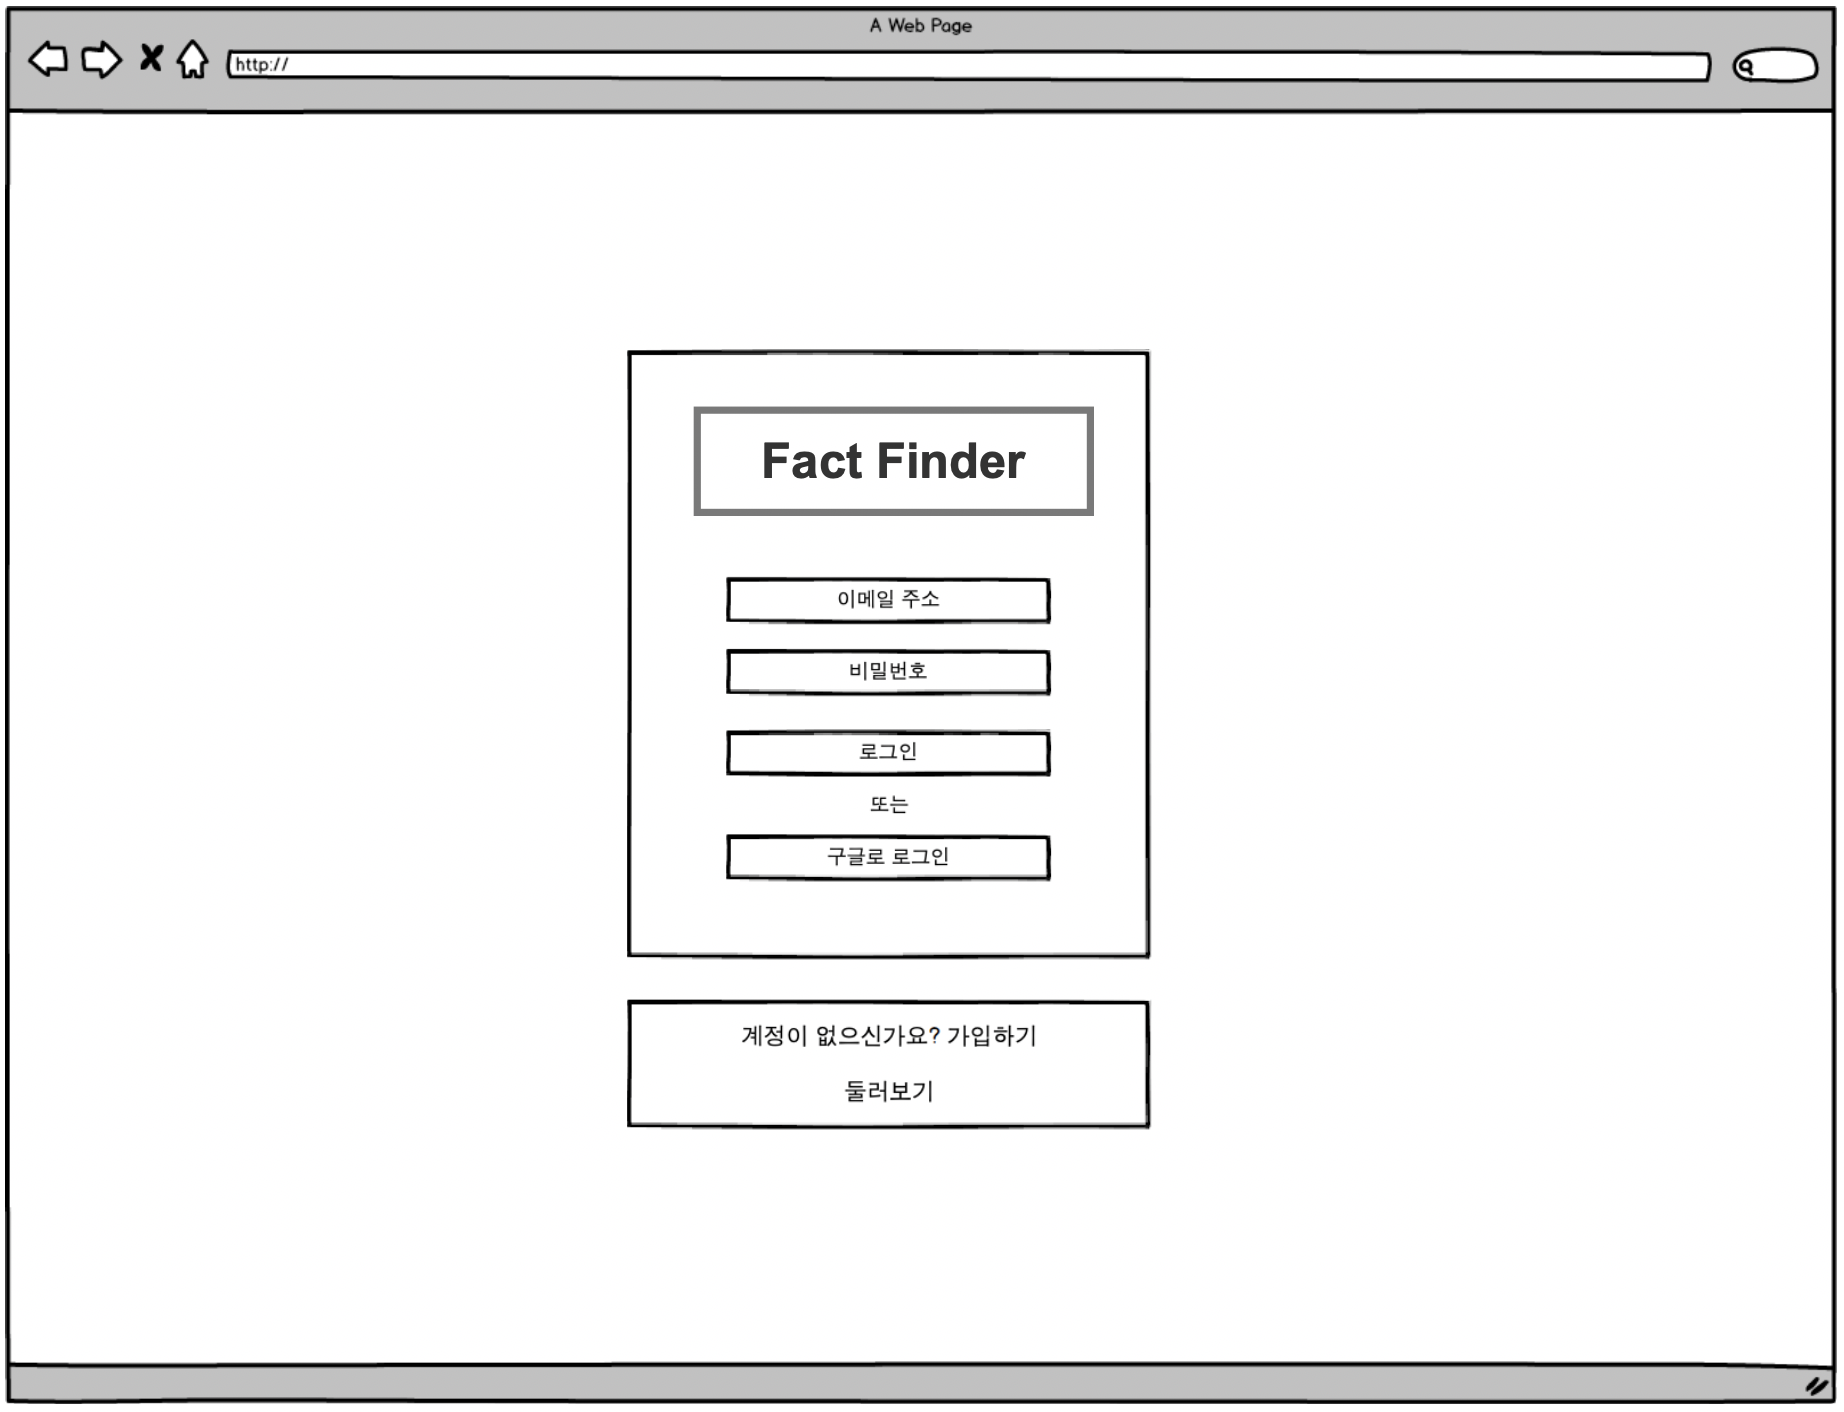
\includegraphics[width=89mm,scale=0.5]{fig/1.png}}
	\caption{Log-in}
	\label{fig}
	\end{figure}
    	\item \textit{Log-in: }Log-in page is a first page that users can see when they enter to our website. The user have to fill out their e-mail and password in this page.  If username and password are match to our database, user can log in our web page to use our personalized system. If users succeed to log in, they can be identified through the internal identifying process so that they can move into the main page . Although, they bump into the failure message if the password is wrong. furthermore, if they enter wrong password  over five times, their accounts are locked so that they have to certificate their identity through contact address such as e-mail, phone number to get certification number to unlock their accounts.  If they want to use our service without login, they can press “looking around button”. In this case, they can use our service without our “subscribing function of interested politician. Also they can choose “Sign up button” to get into the sign up page  if they want to sign up to our service.\\
    	\begin{figure}[htbp]
	\centerline{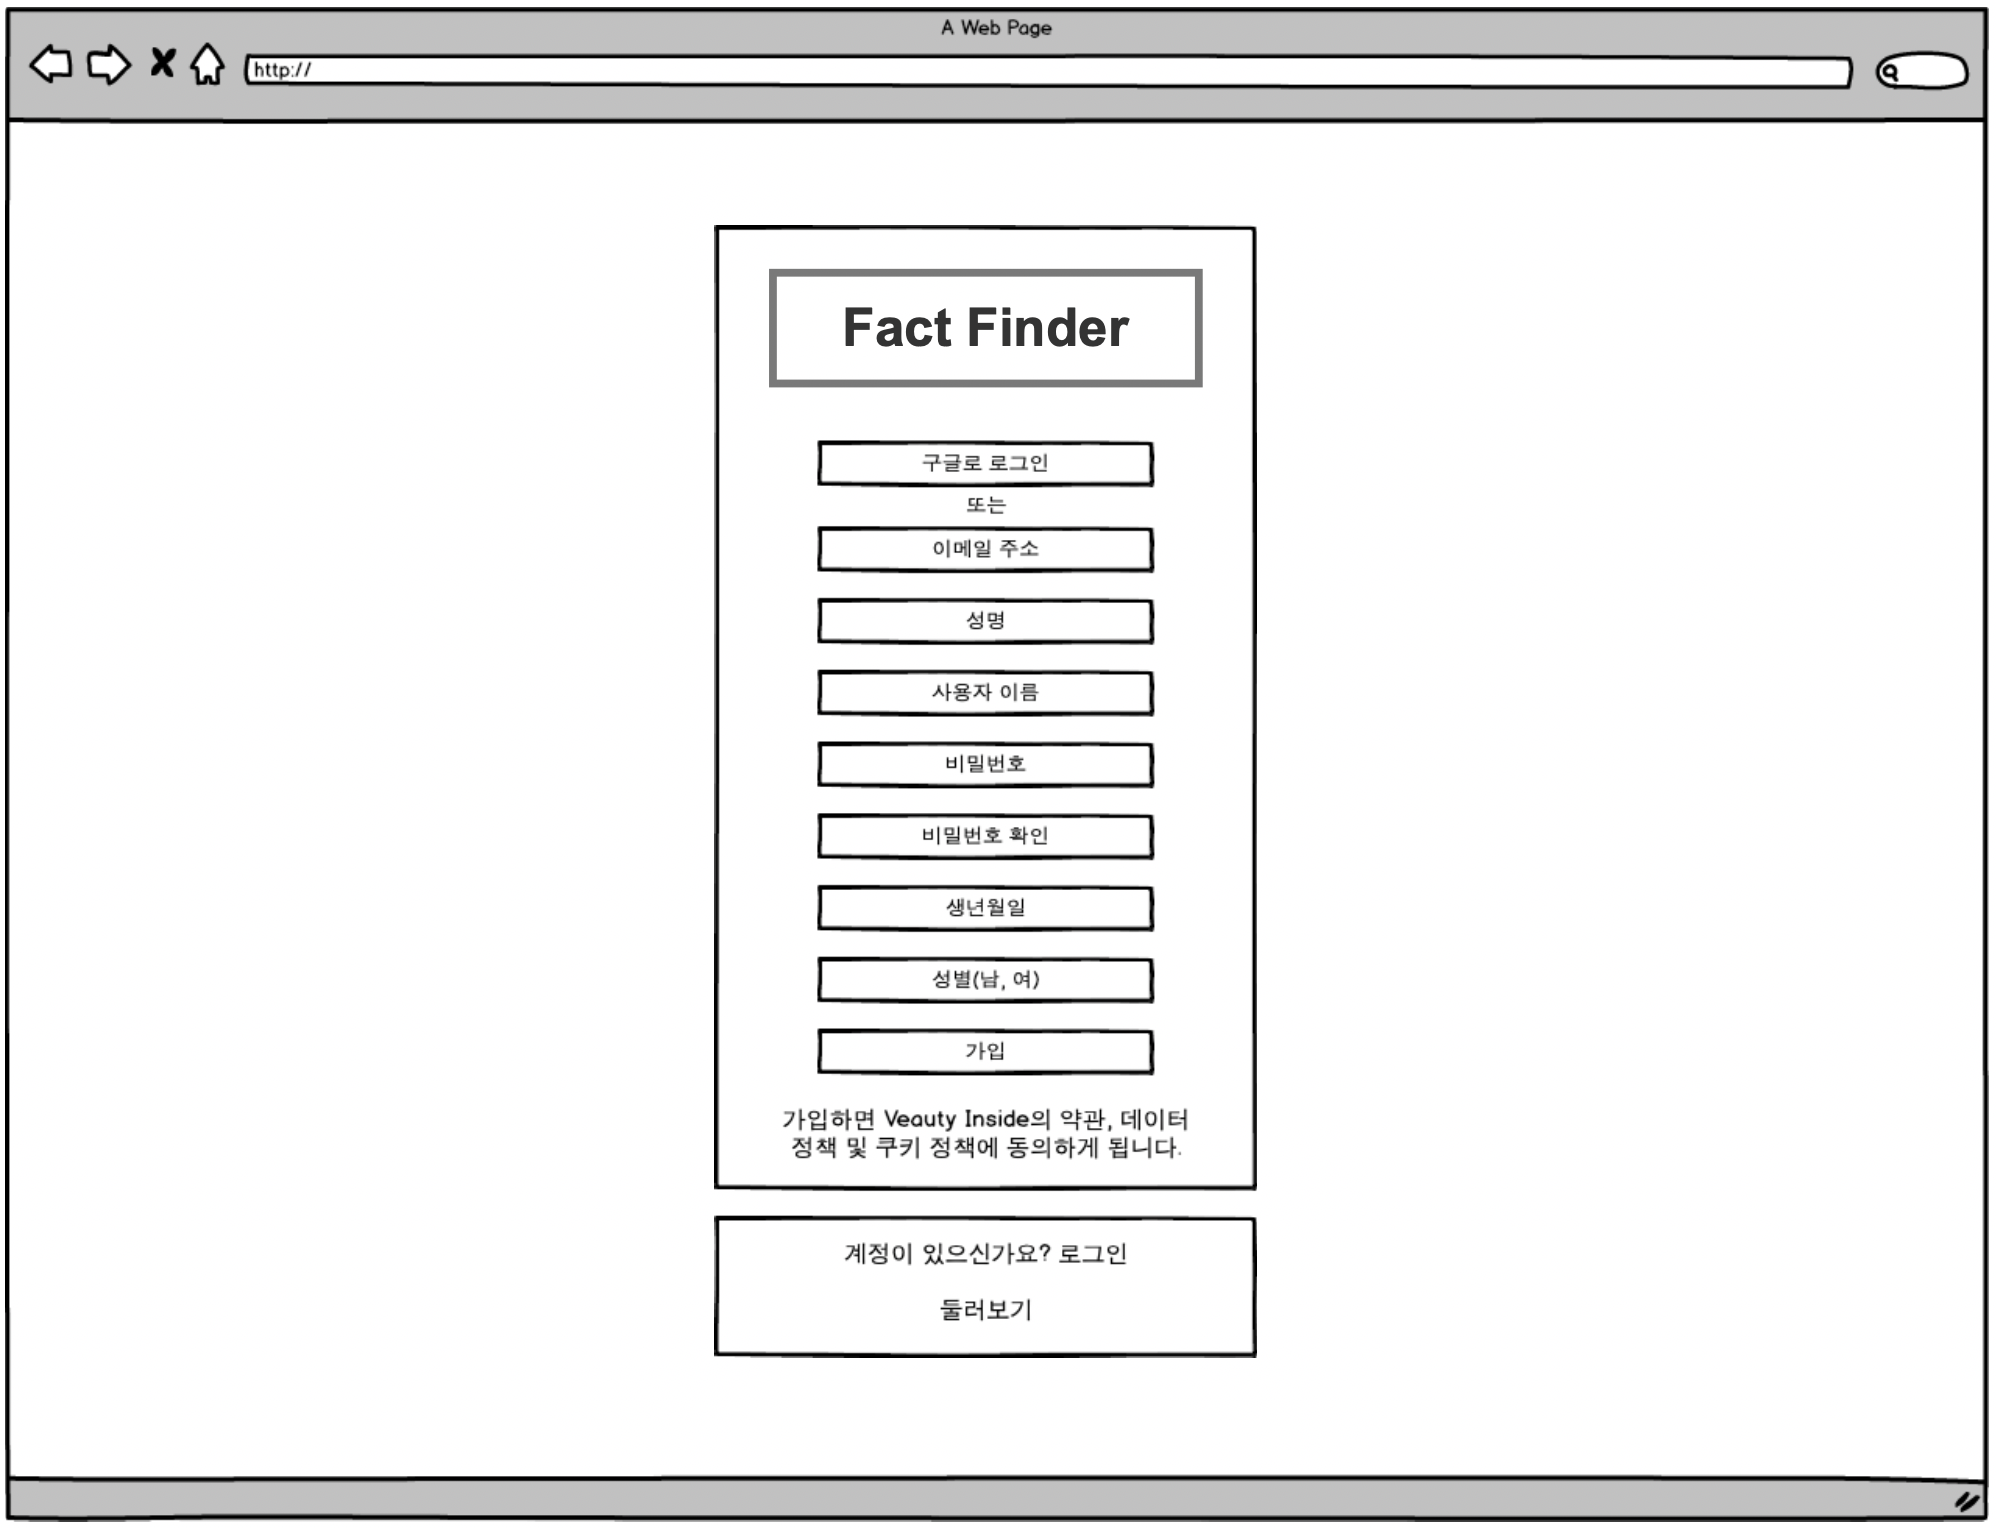
\includegraphics[width=89mm,scale=0.5]{fig/2.png}}
	\caption{sign-up}
	\label{fig}
	\end{figure}
	\\
	\\
	\\
	\\
        \item \textit{sign-up: }This page requires user to users’ information  such as E-mail, Username, Nickname, password, birth date, sex. These information are submitted to our database. Also, user must agree on our services’ terms,data, cookie policy. User can sign in into our page if they finish their forming information process. Furthermore, User can sign up through Kakao talk, Google, Naver ID certificating processes. If they want to use our service without login, they can press “looking around button”. In this case, they can use our service without our “subscribing function of interested politician. Also they can choose “Sign up button” to get into the sign up page  if they want to sign up to our service.\\
         \item \textit{ID/PW search: }If the user forget about their ID or Password, they can find theirs through this page. Through the information saved on our database, user can certificate themselves by sending certification number to their E-mail,  phone number, or I-PIN. User should change their password after this function.\\
    \end{enumerate}
    
    \item \textit {Main Page: }
    
The main page is a key feature of this service. Users can search for detailed information about minutes. To concrete this, the following functions are implemented.\\
\\navigation bar: it contains several components of the application and user can can navigate to the selected page by selecting the list. nav bar consists of the following items and is linked to each item.\\
    \begin{enumerate}
    	\item \textit{Looking up function about meeting contents per agenda	:} \\
	
	     \begin{enumerate}
	     
	\begin{figure}[htbp]
	\centerline{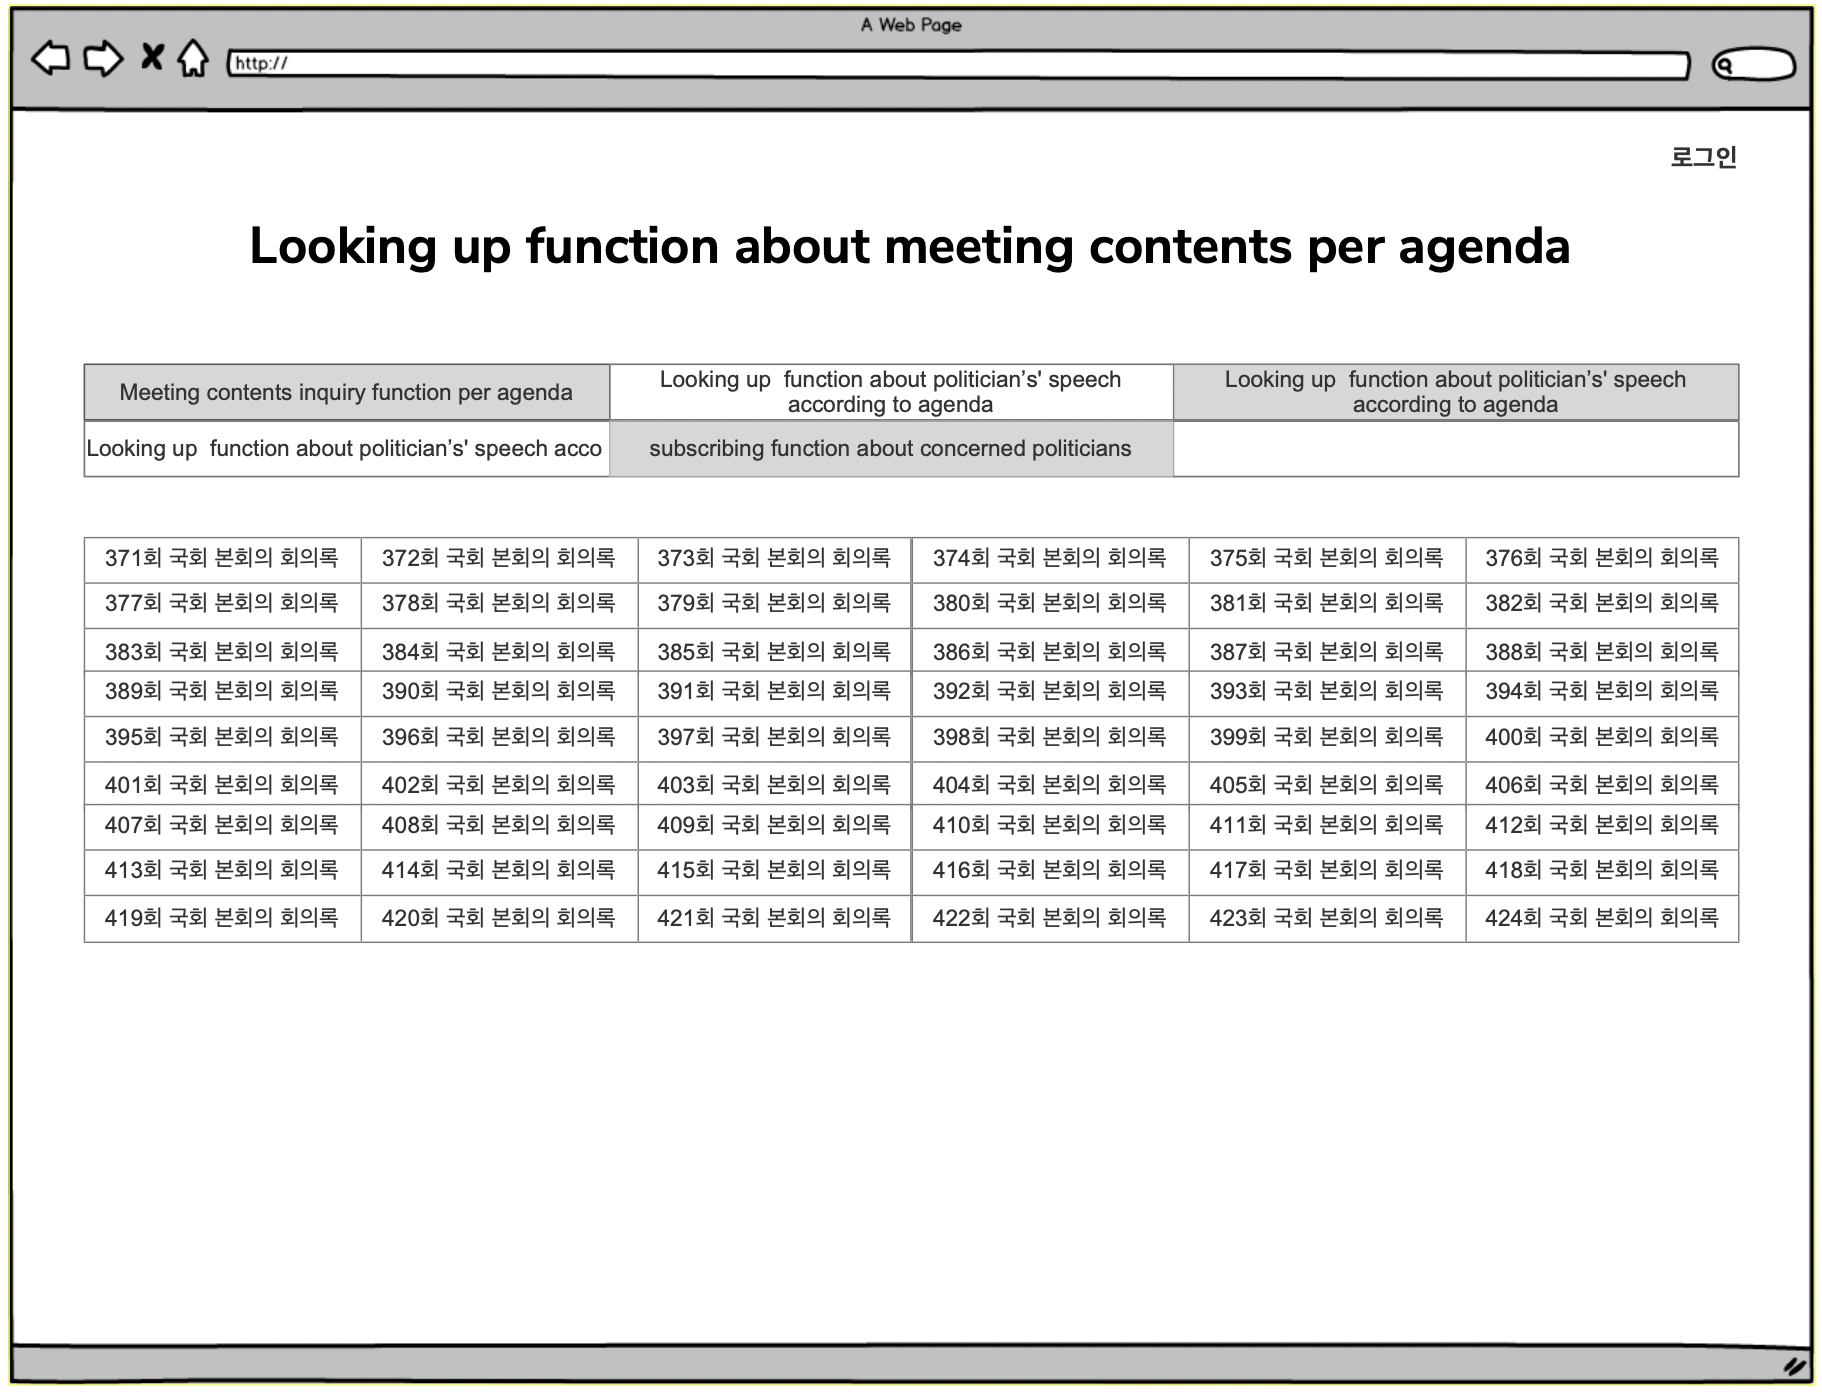
\includegraphics[width=89mm,scale=0.5]{fig/3.png}}
	\caption{Looking up function about meeting contents per agenda}
	\label{fig}
	\end{figure}     
    	\item \textit{} This function consists of three pages. In first page, it shows assembly minutes list. Minutes list that is classified periodically includes monthly, weekly, and certain time period setting function. Because of this, user can search the record of the past and view minutes in certain date.\\
	
		\begin{figure}[htbp]
	\centerline{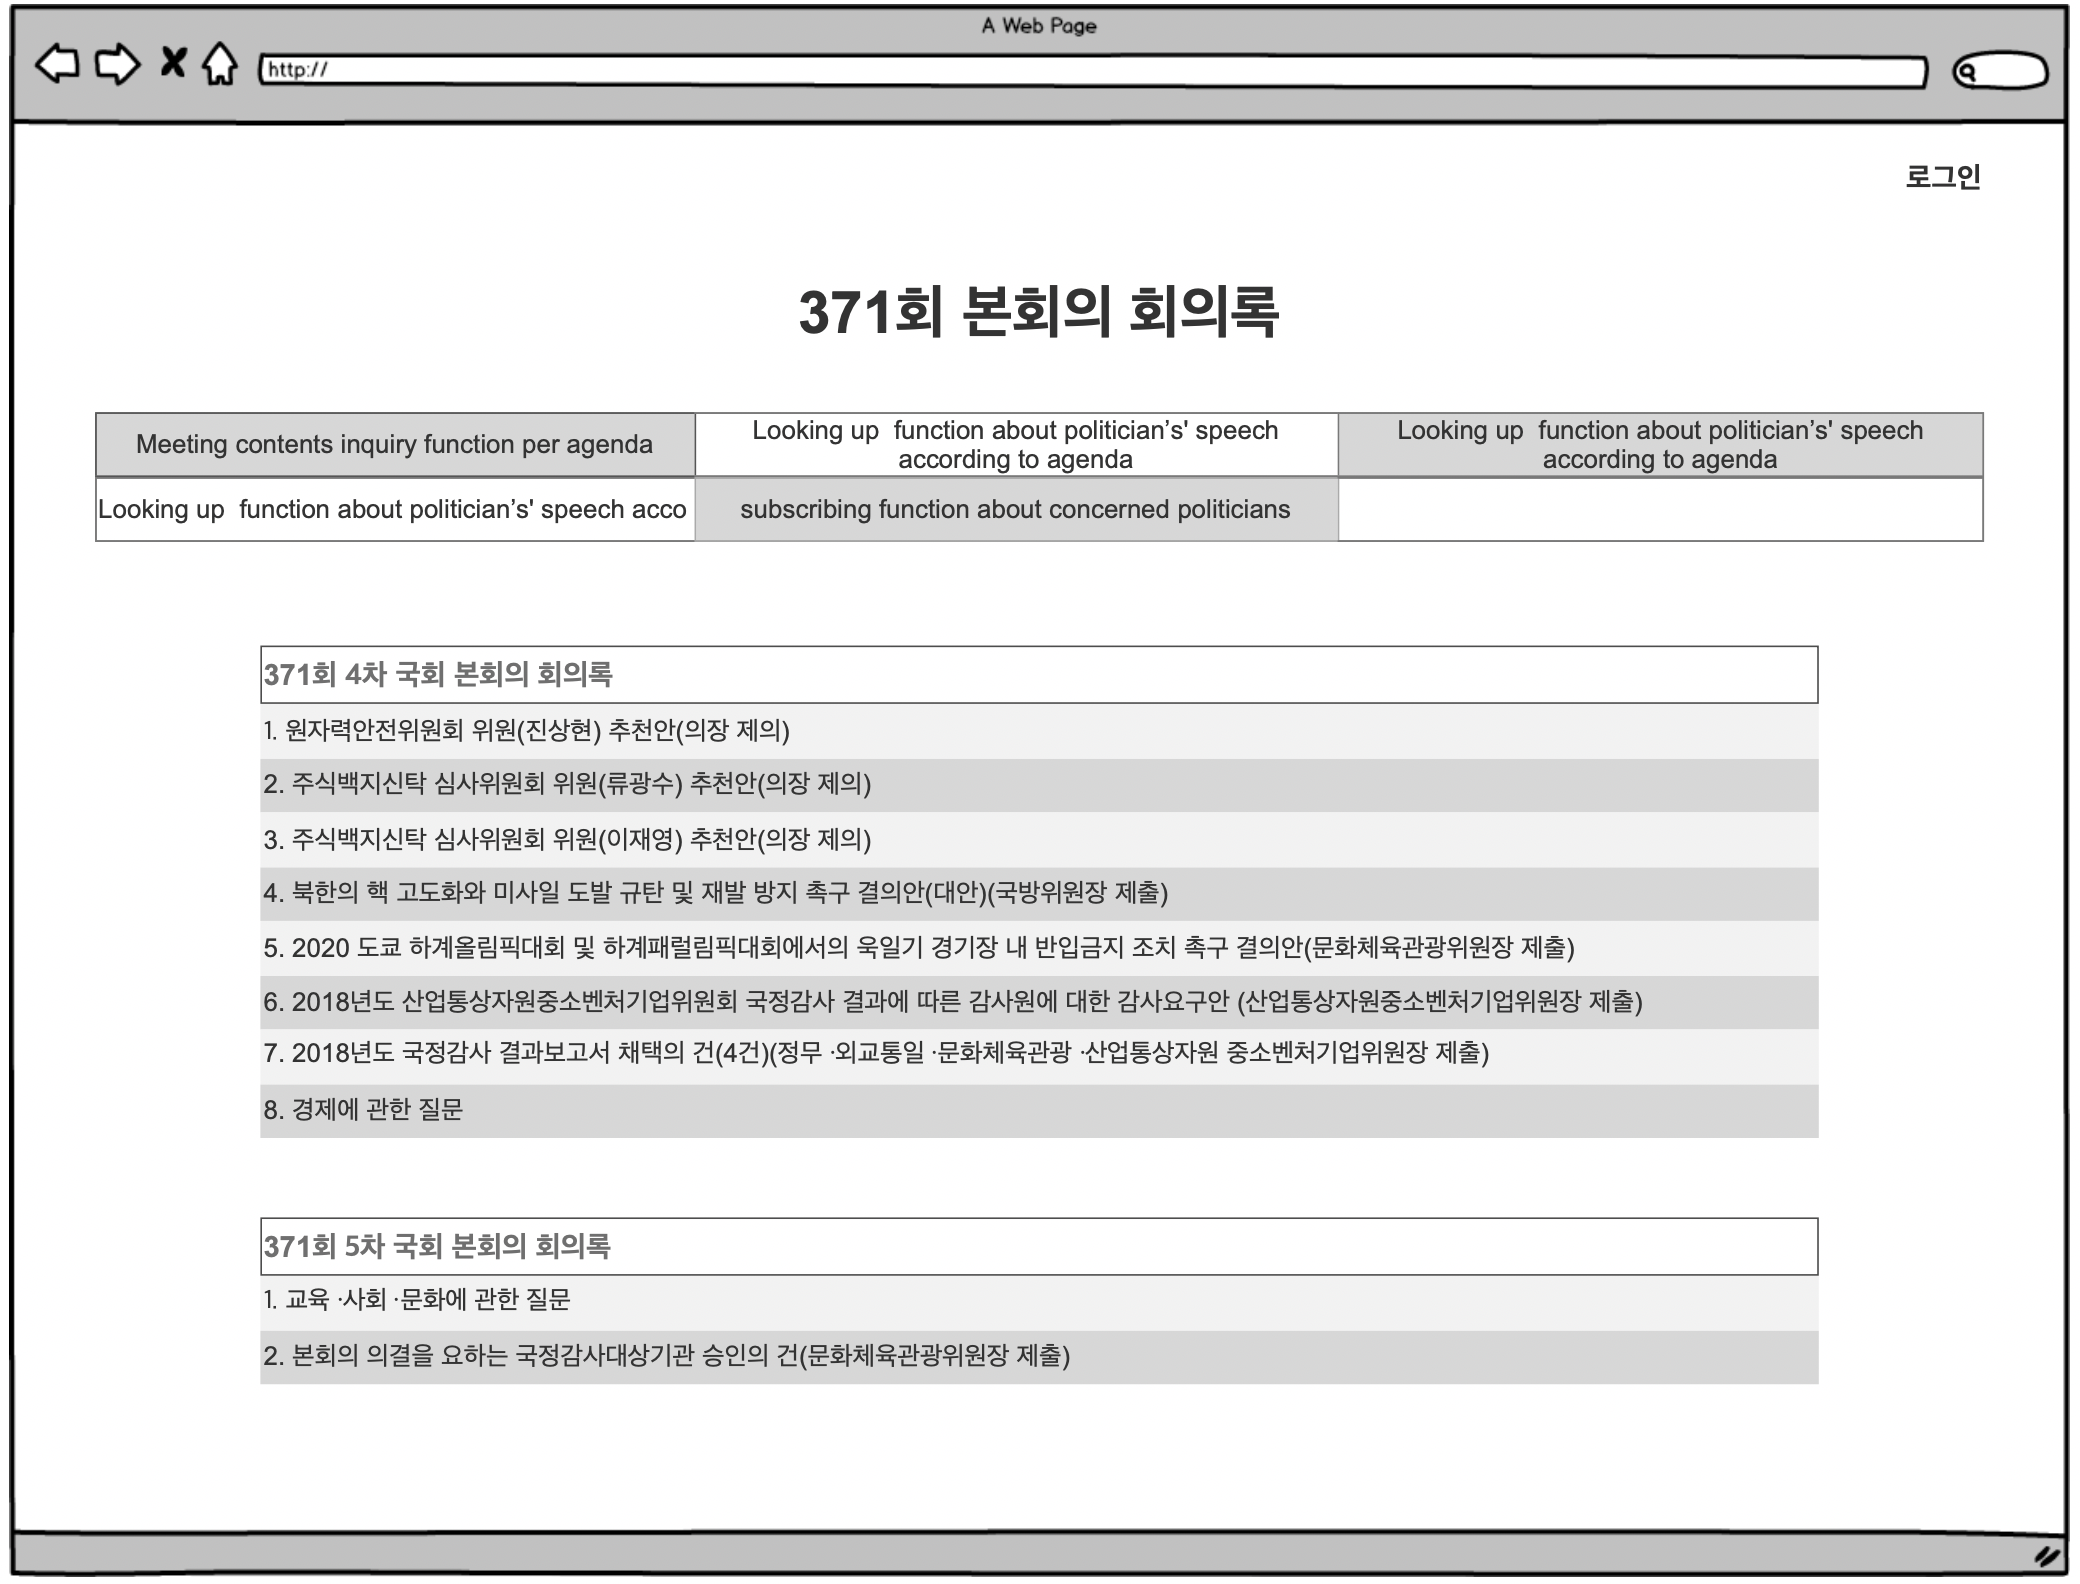
\includegraphics[width=89mm,scale=0.5]{fig/4.png}}
	\caption{Looking up function about meeting contents per agenda}
	\label{fig}
	\end{figure}     
	
        \item \textit{} In Second page, It consists of each minutes’ count number and agendas. In the big table, it shows each count number, specifically, each table contains what agendas are discussed in that congress meeting. If user wants to search specific agenda, he can just view that  by clicking that agenda. He can move onto the detail page. \\
        
        		\begin{figure}[htbp]
	\centerline{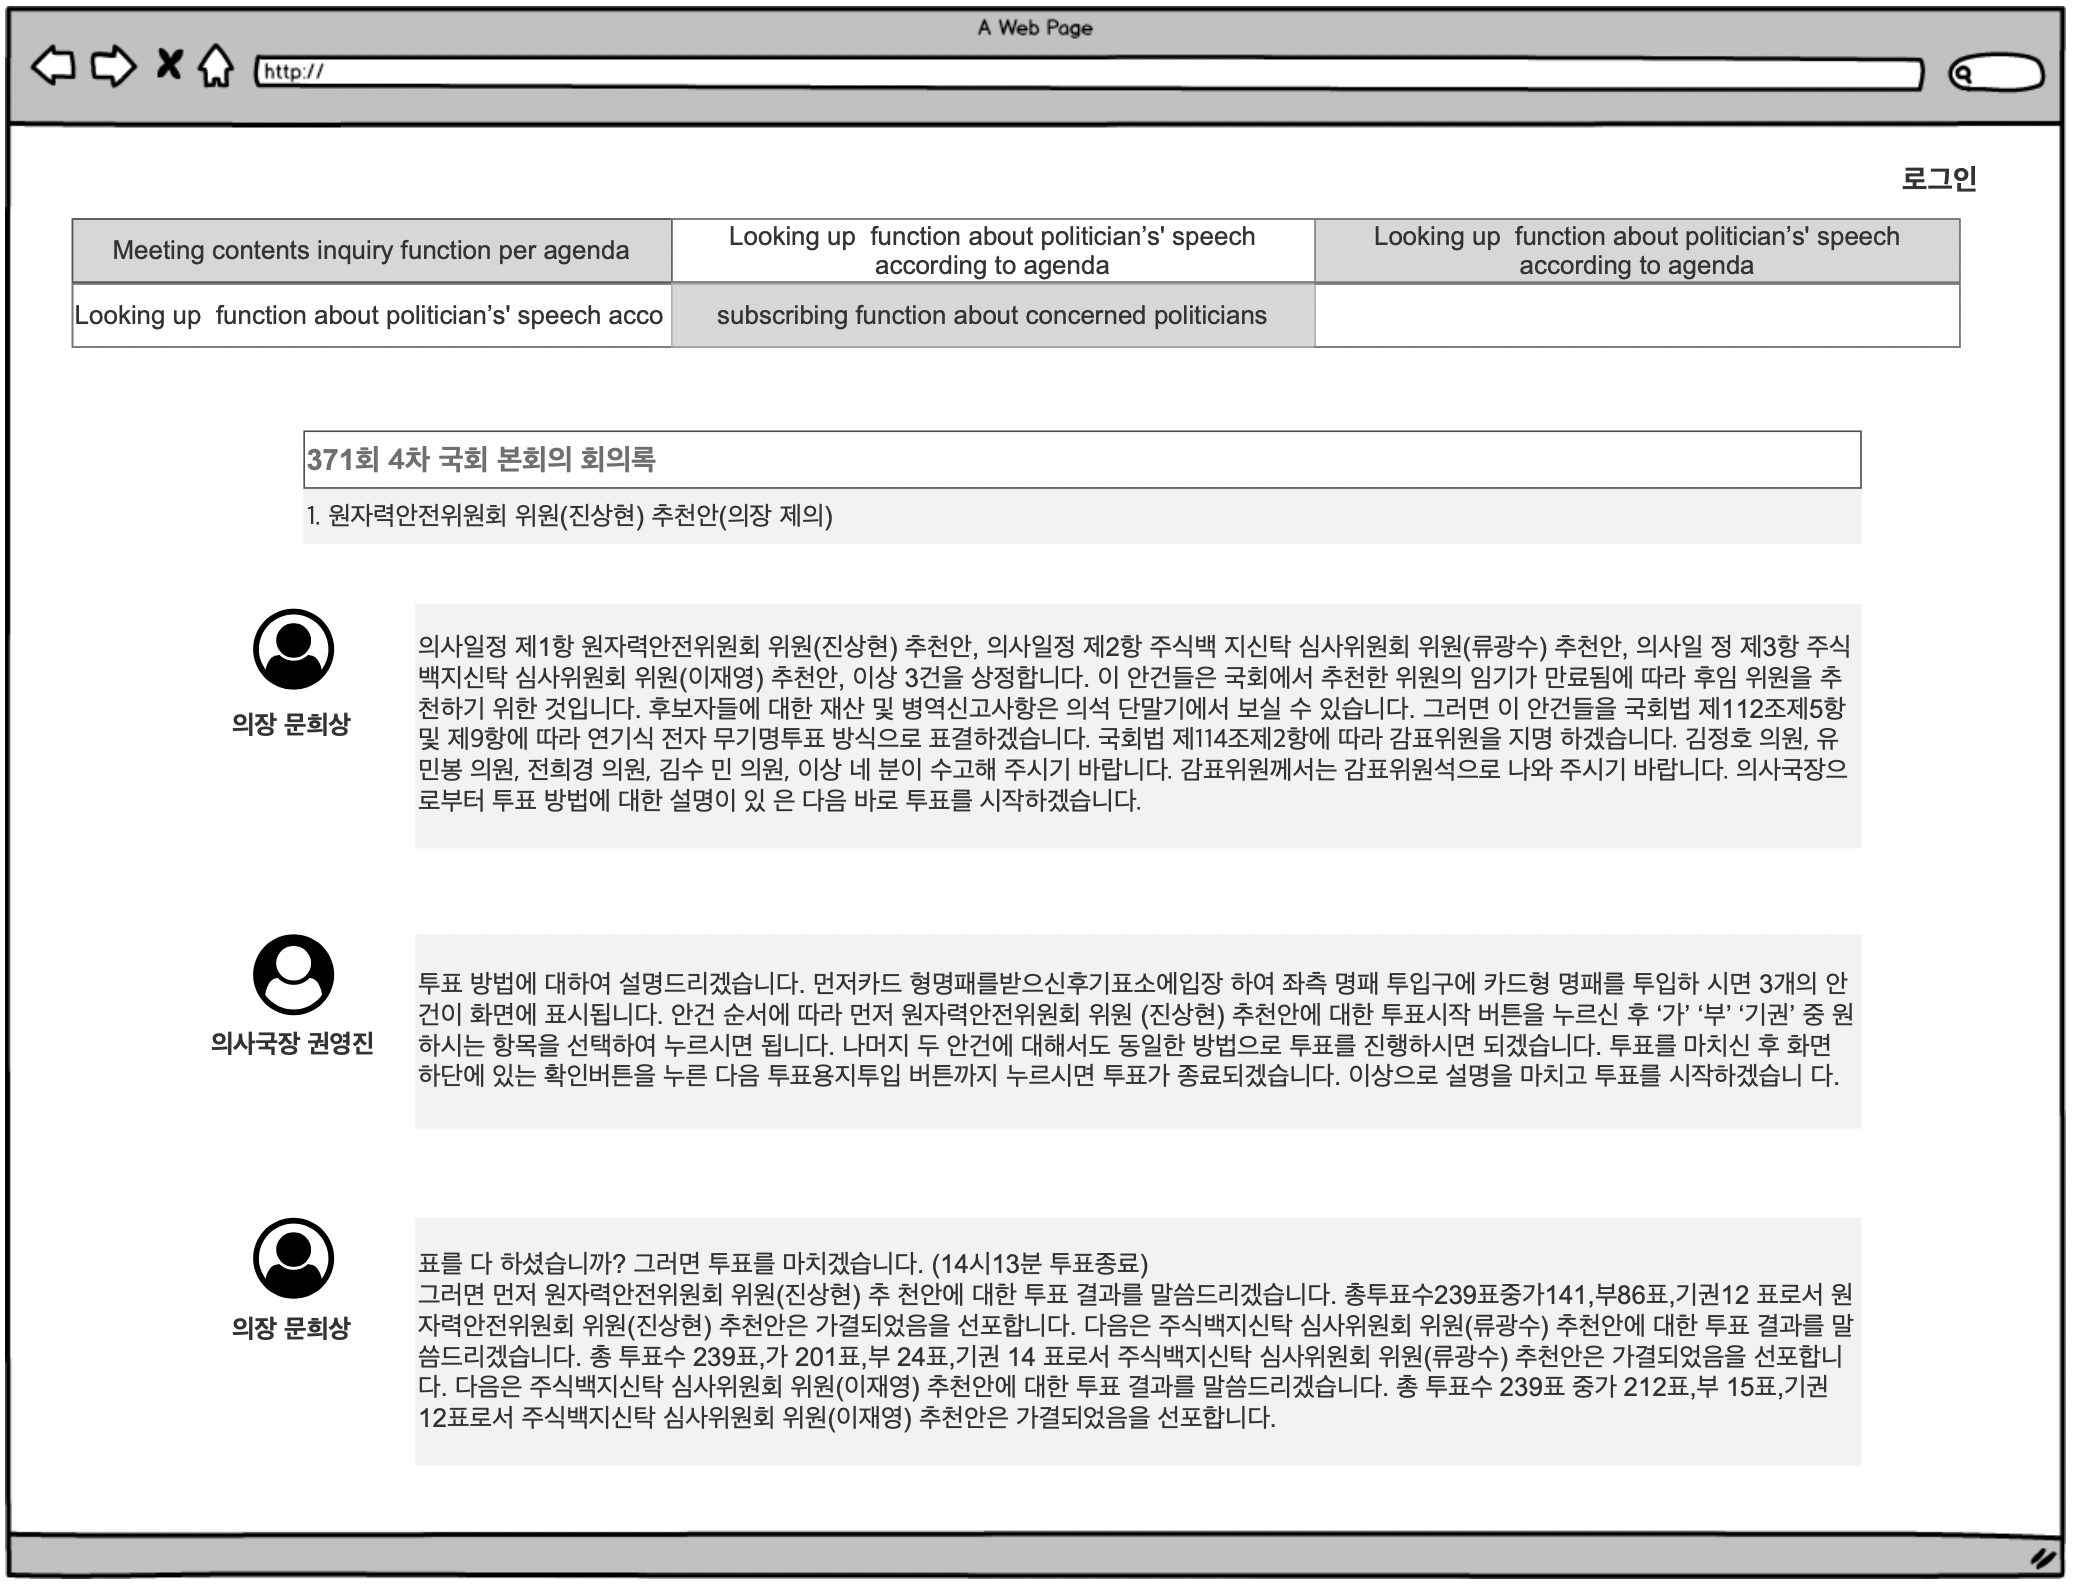
\includegraphics[width=89mm,scale=0.5]{fig/5.png}}
	\caption{Looking up function about meeting contents per agenda}
	\label{fig}
	\end{figure}     

         \item \textit{} In third page, it shows detail page that is chosen by the user. It looks like social messenger, talking each other like shown above. Specifically, The politician’s image is attached and his or her speech is surrounded by a box.\\
           \end{enumerate}
           
                   		\begin{figure}[htbp]
	\centerline{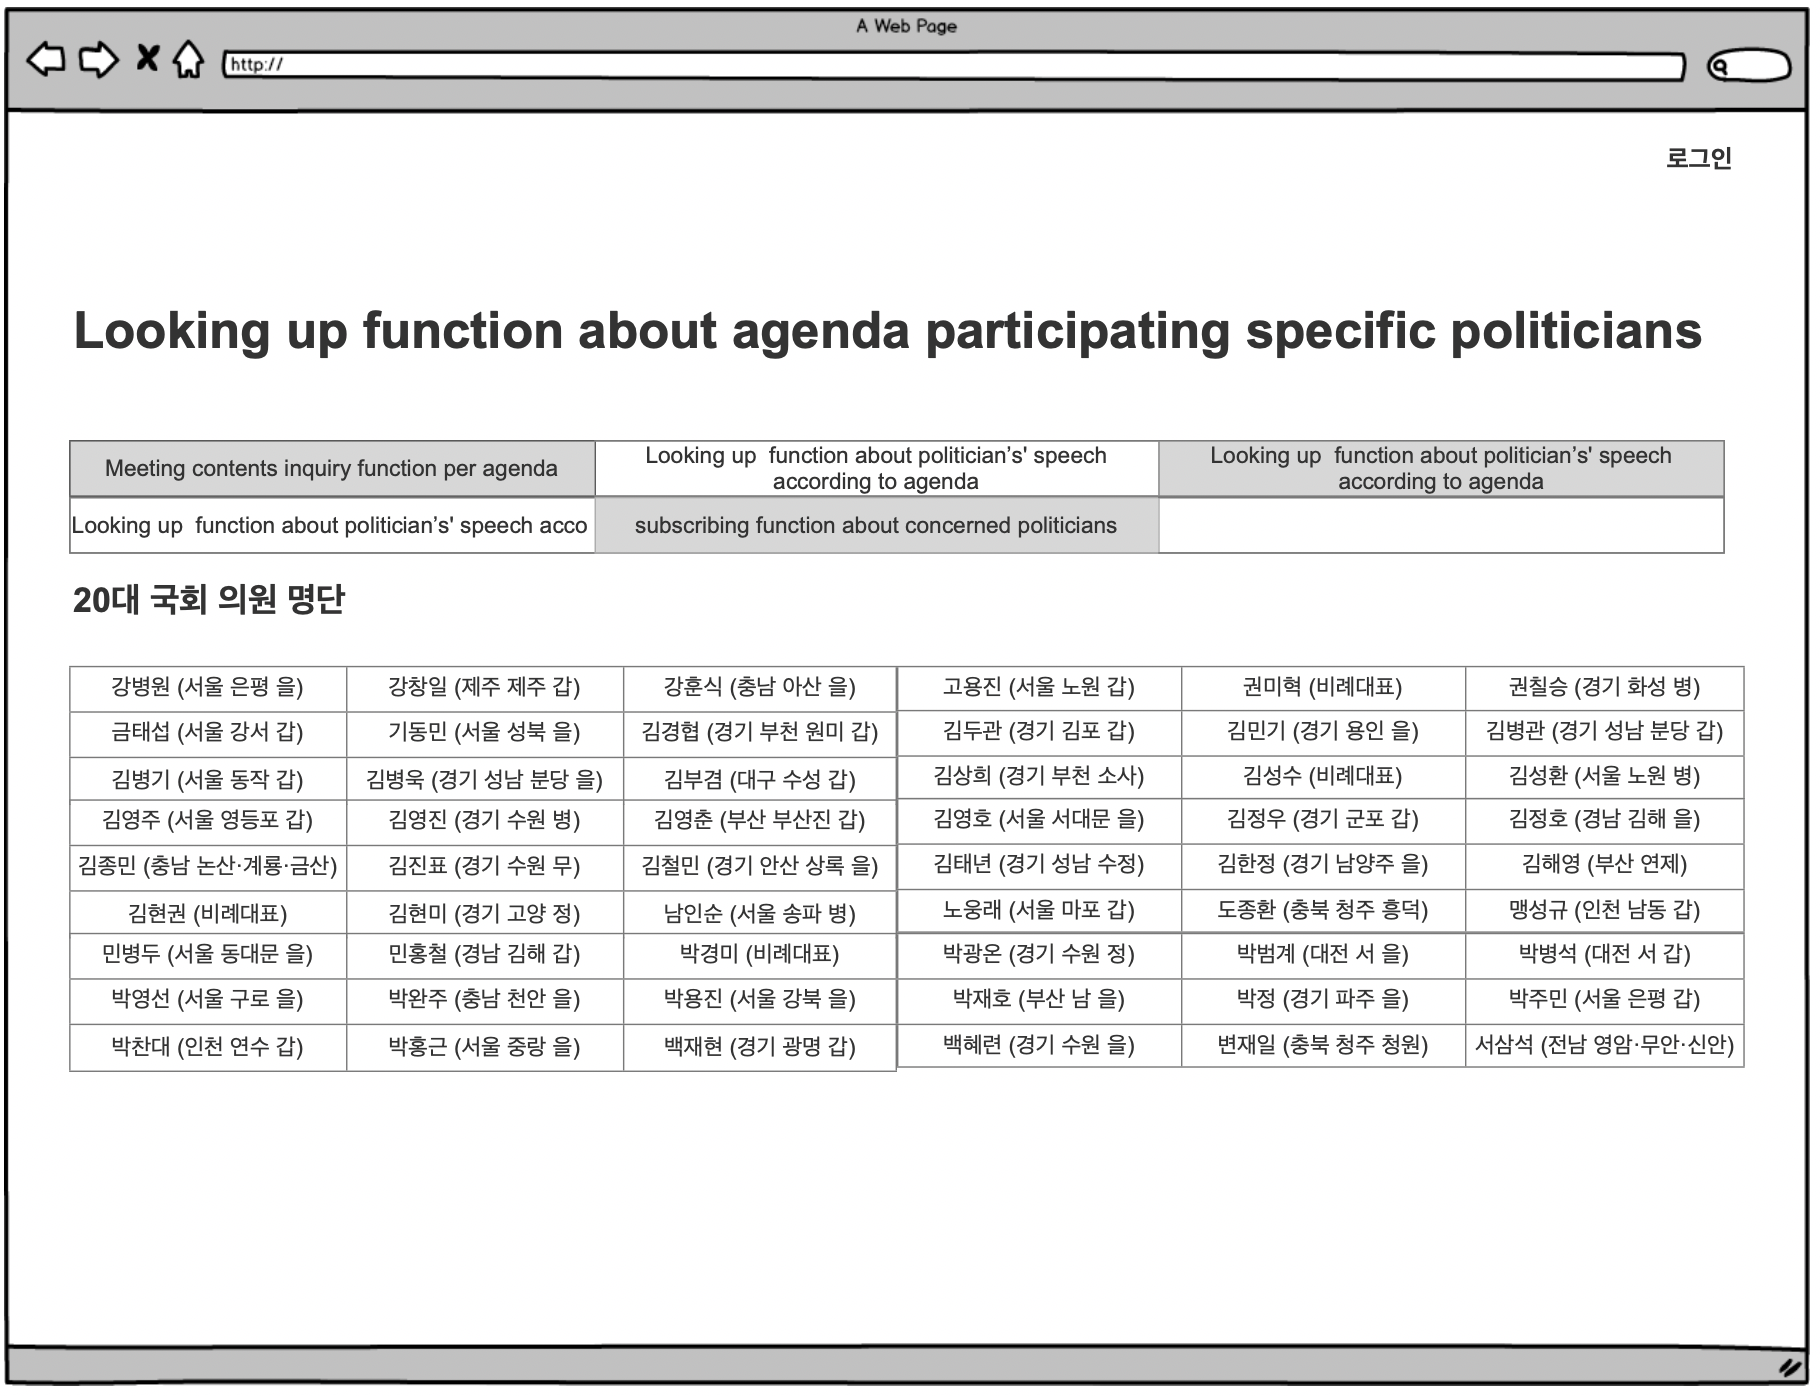
\includegraphics[width=89mm,scale=0.5]{fig/6.png}}
	\caption{Looking up function about agenda participating specific politicians}
	\label{fig}
	\end{figure}     
           
        \item \textit{Looking up function about agenda participating specific politicians: }  \\
        	     \begin{enumerate}

    	\item \textit{} In this page, user can view specific politicians’ participated agenda. User can view current members of assembly along with where they’re belonged to. If user click a member, they can move onto the page that politician’s commented agendas. This page is implemented as separated function as third below, “Looking up  function about politician’s' speech according to agenda”. \\
        \item \textit{} If user wants to follow specific politician what they did in assembly  on and on, they can click subscribe button in the member box. In this case, user can check what they saved in the fourth function, “Looking up function about subscribing politics”. This function is activated only if the user was logged in.\\
           \end{enumerate}
           
                              		\begin{figure}[htbp]
	\centerline{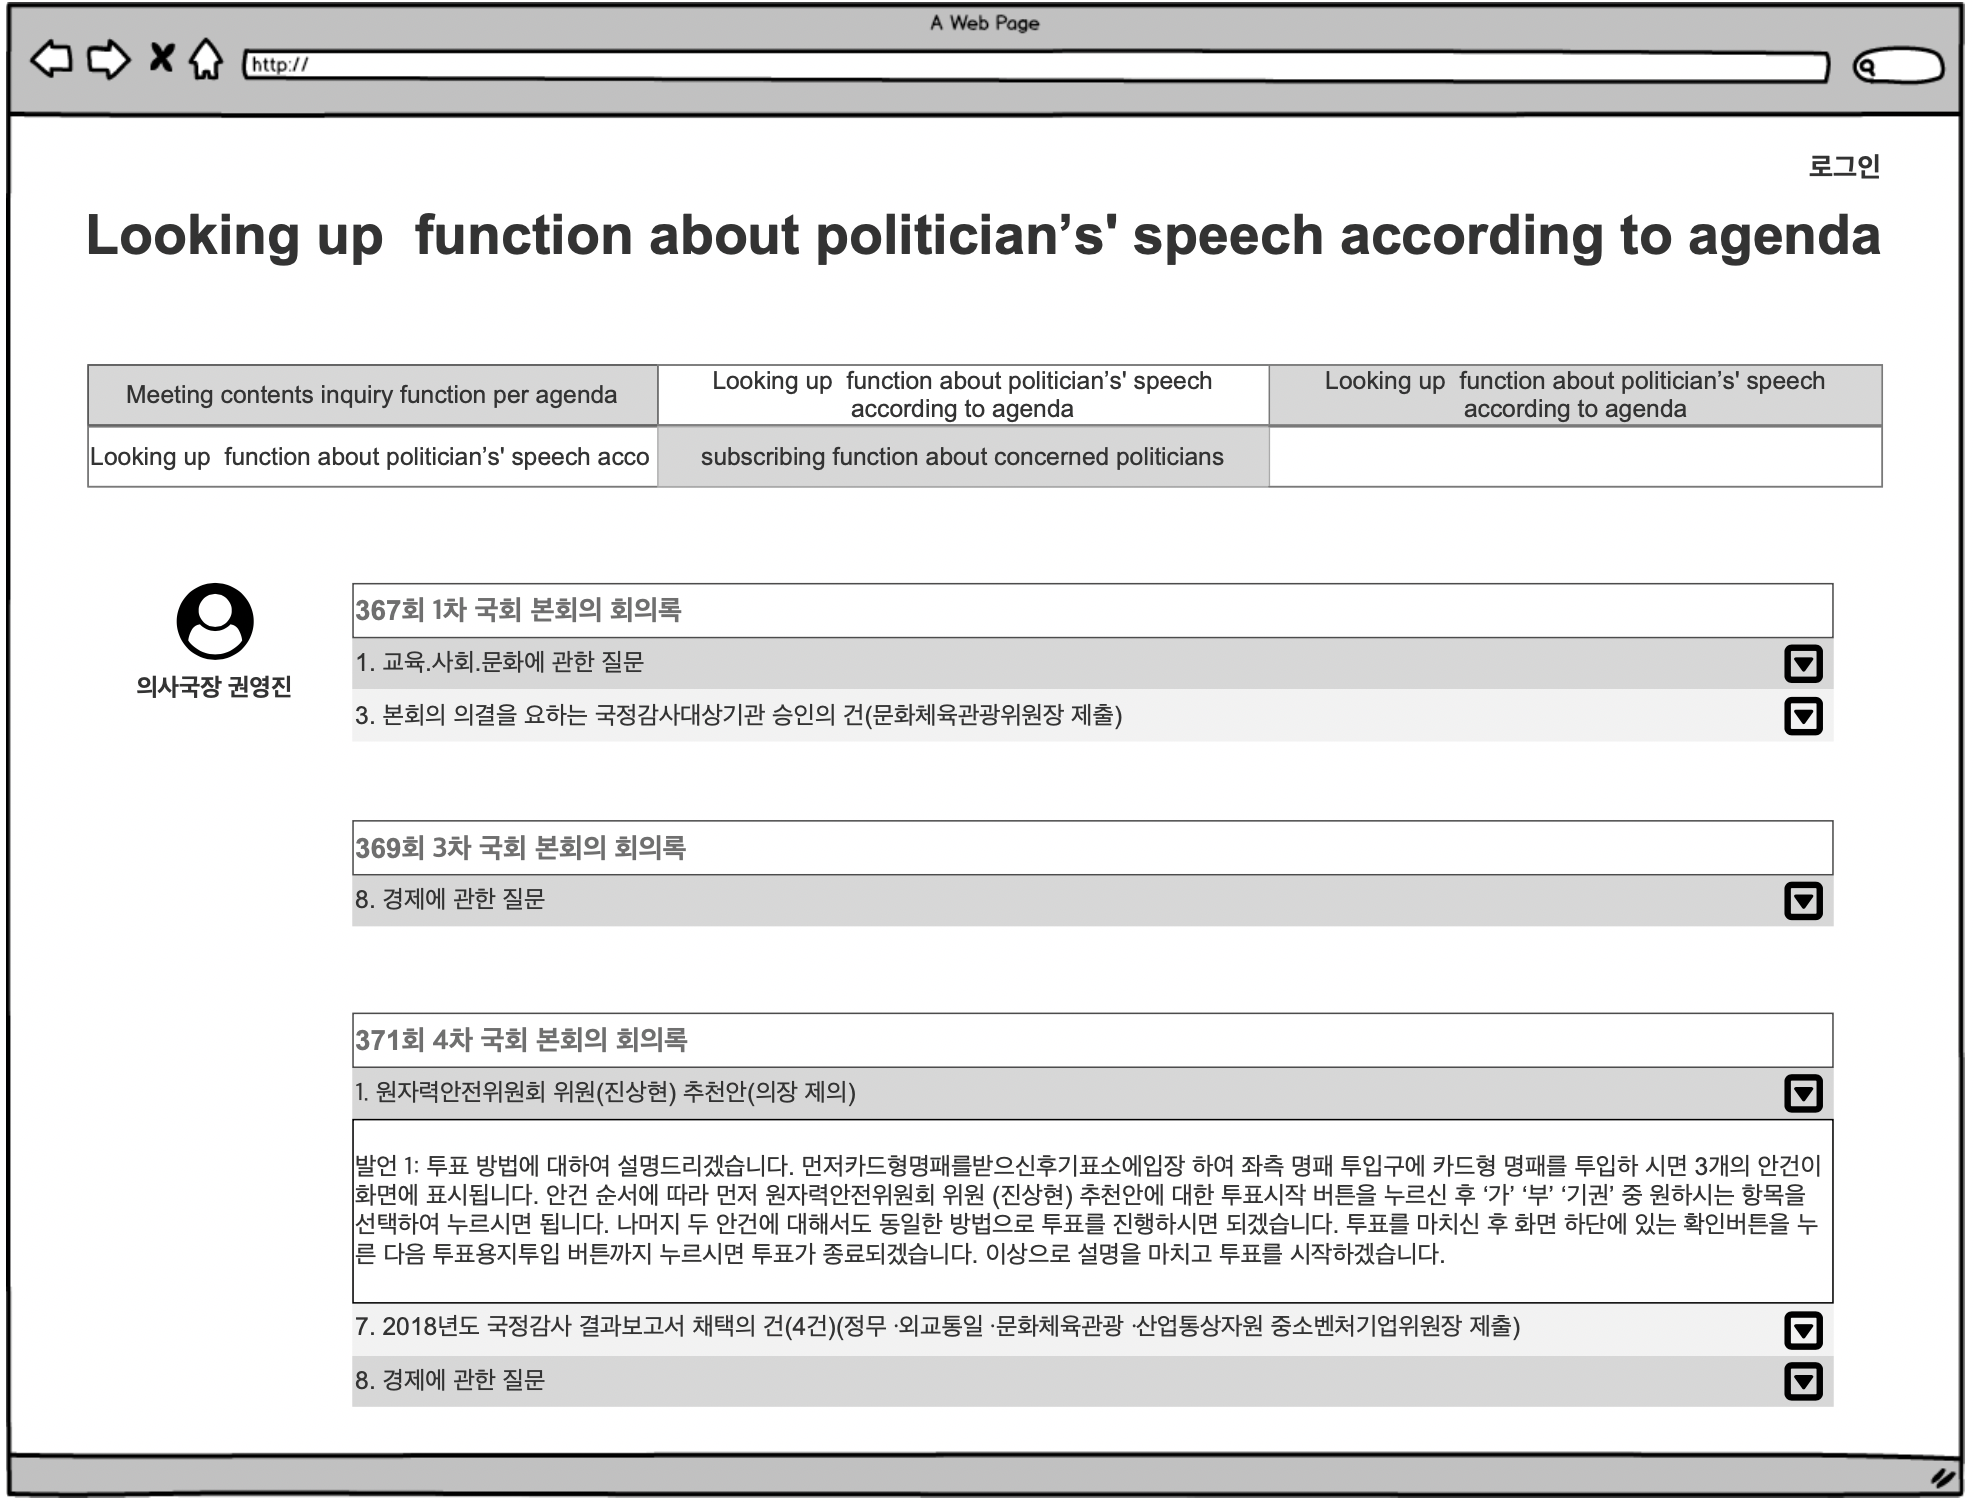
\includegraphics[width=89mm,scale=0.5]{fig/7.png}}
	\caption{Looking up  function about politician’s' speech according to agenda}
	\label{fig}
	\end{figure}     
     
        \item \textit{Looking up  function about politician’s' speech according to agenda:}  \\
        	     \begin{enumerate}

    	\item \textit{} If user selected or searched to specific politician, they can view this page. In this page, User can see specific politician’s participated agenda. Each table is consisted of the name of the assembly minutes, and details are filled with that politician’s participated agenda. If user wants to view what they spoke specifically at that agenda, they can click the pointing down arrow button. the pop-up box shows the politician’s speech, and its contents are separated with numbers like ‘speech1, speech2’.\\
        \item \textit{} If user wants to follow specific politician what they did in assembly  on and on, they can click subscribe button in the member box. In this case, user can check what they saved in the fourth function, “Looking up function about subscribing politics”. This function is activated only if the user was logged in.\\
           \end{enumerate}

                              		\begin{figure}[htbp]
	\centerline{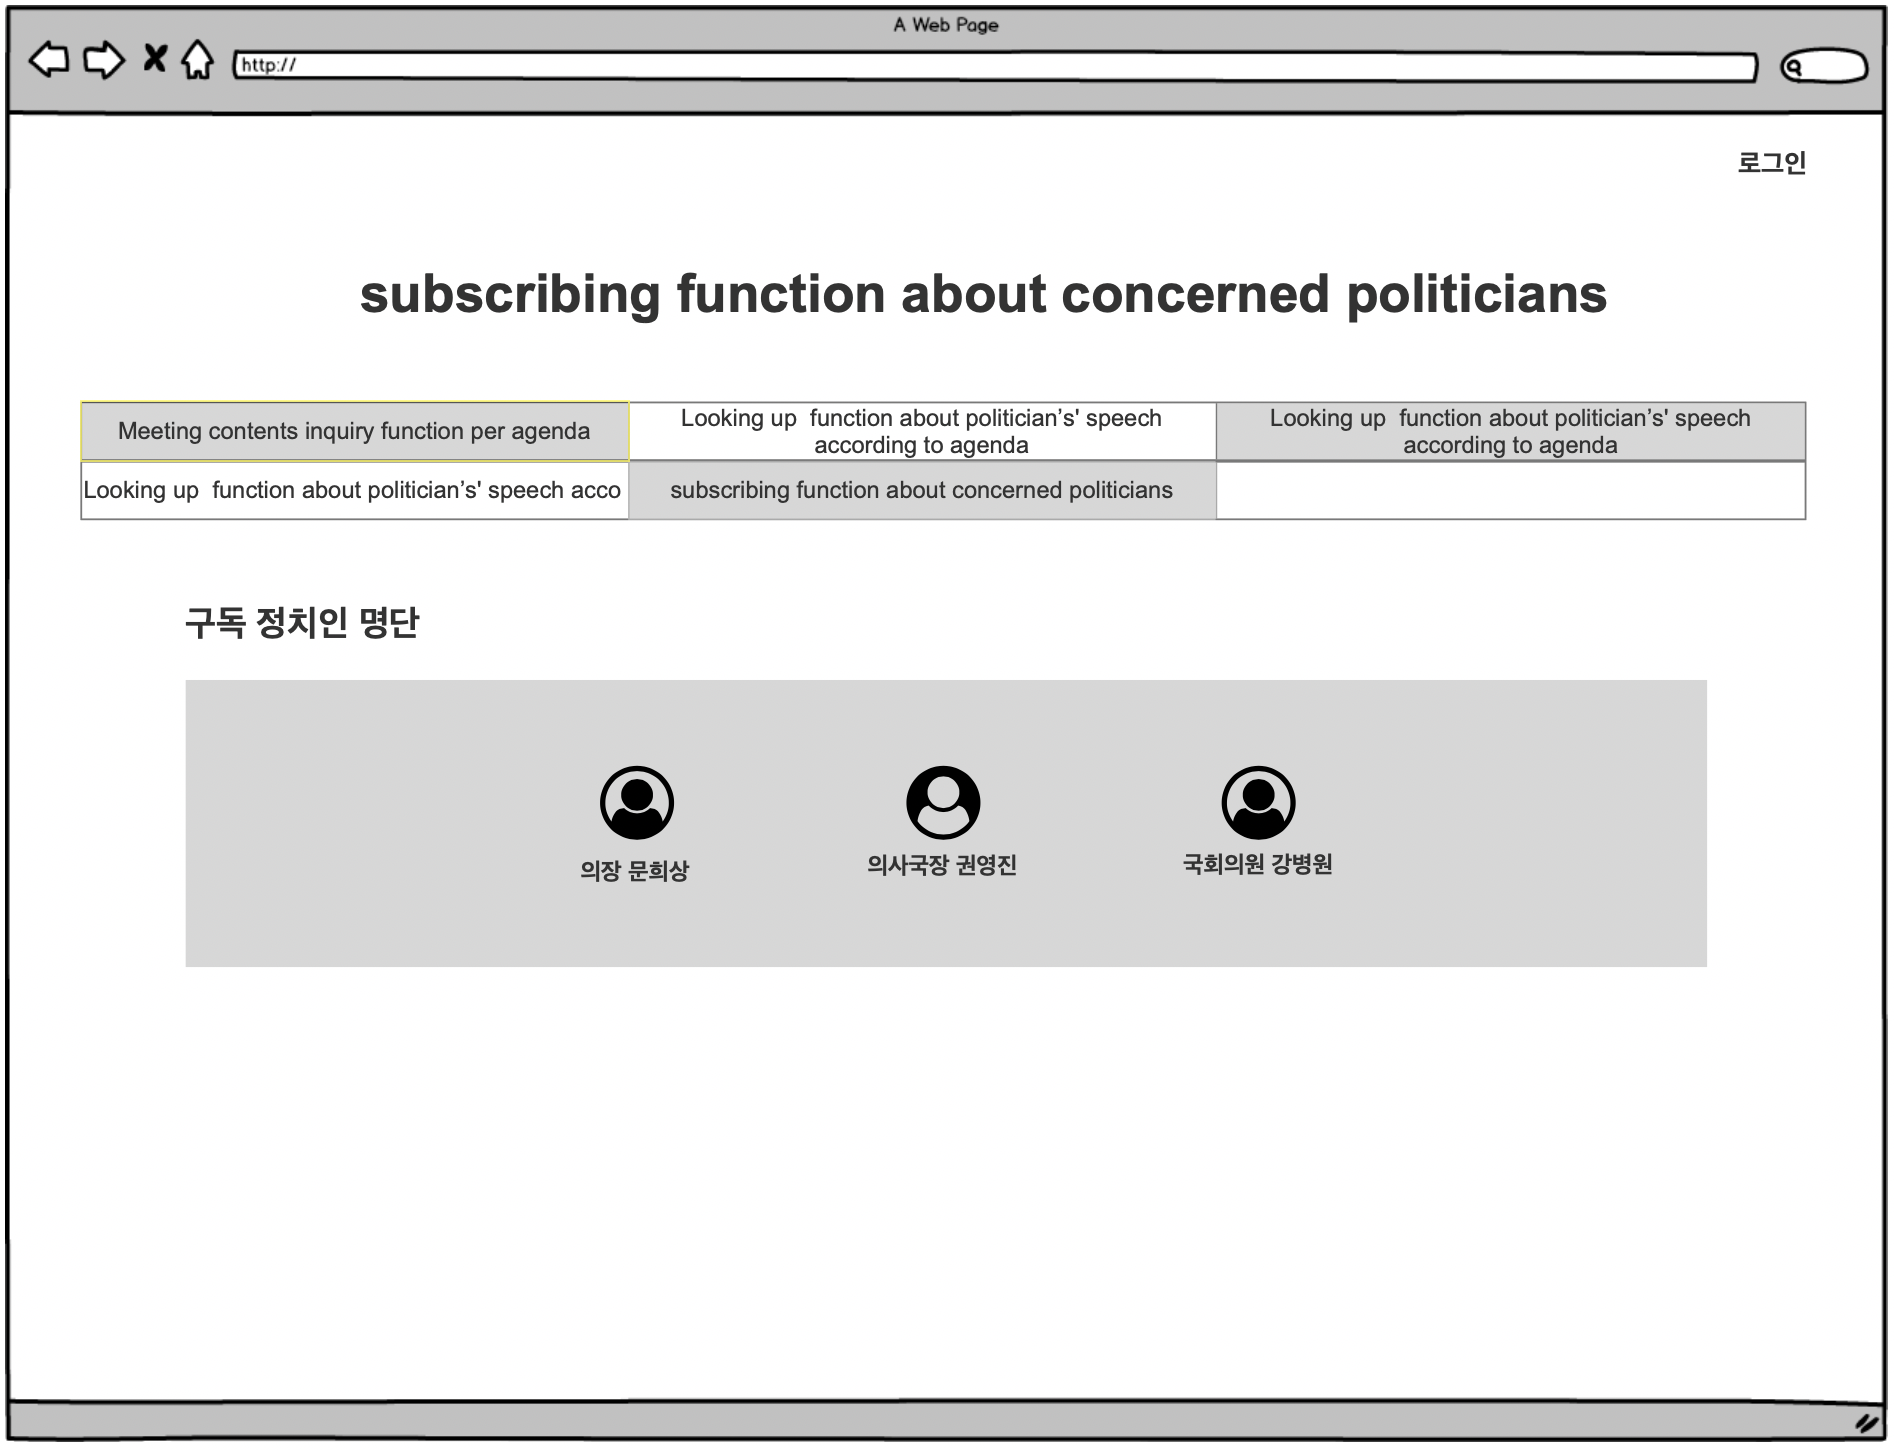
\includegraphics[width=89mm,scale=0.5]{fig/8.png}}
	\caption{Looking up  function about subscribing politicians}
	\label{fig}
	\end{figure}     
    \item \textit {Looking up  function about subscribing politicians: }User can subscribe user’s interested politicians. In this page, user can customize this page by subscribing specific politicians functions implemented above. They can choose their favorite politicians. If the user click the image of politician, they can move onto the third function, “Looking up  function about politician’s' speech according to agenda”.\\
    
                                  		\begin{figure}[htbp]
	\centerline{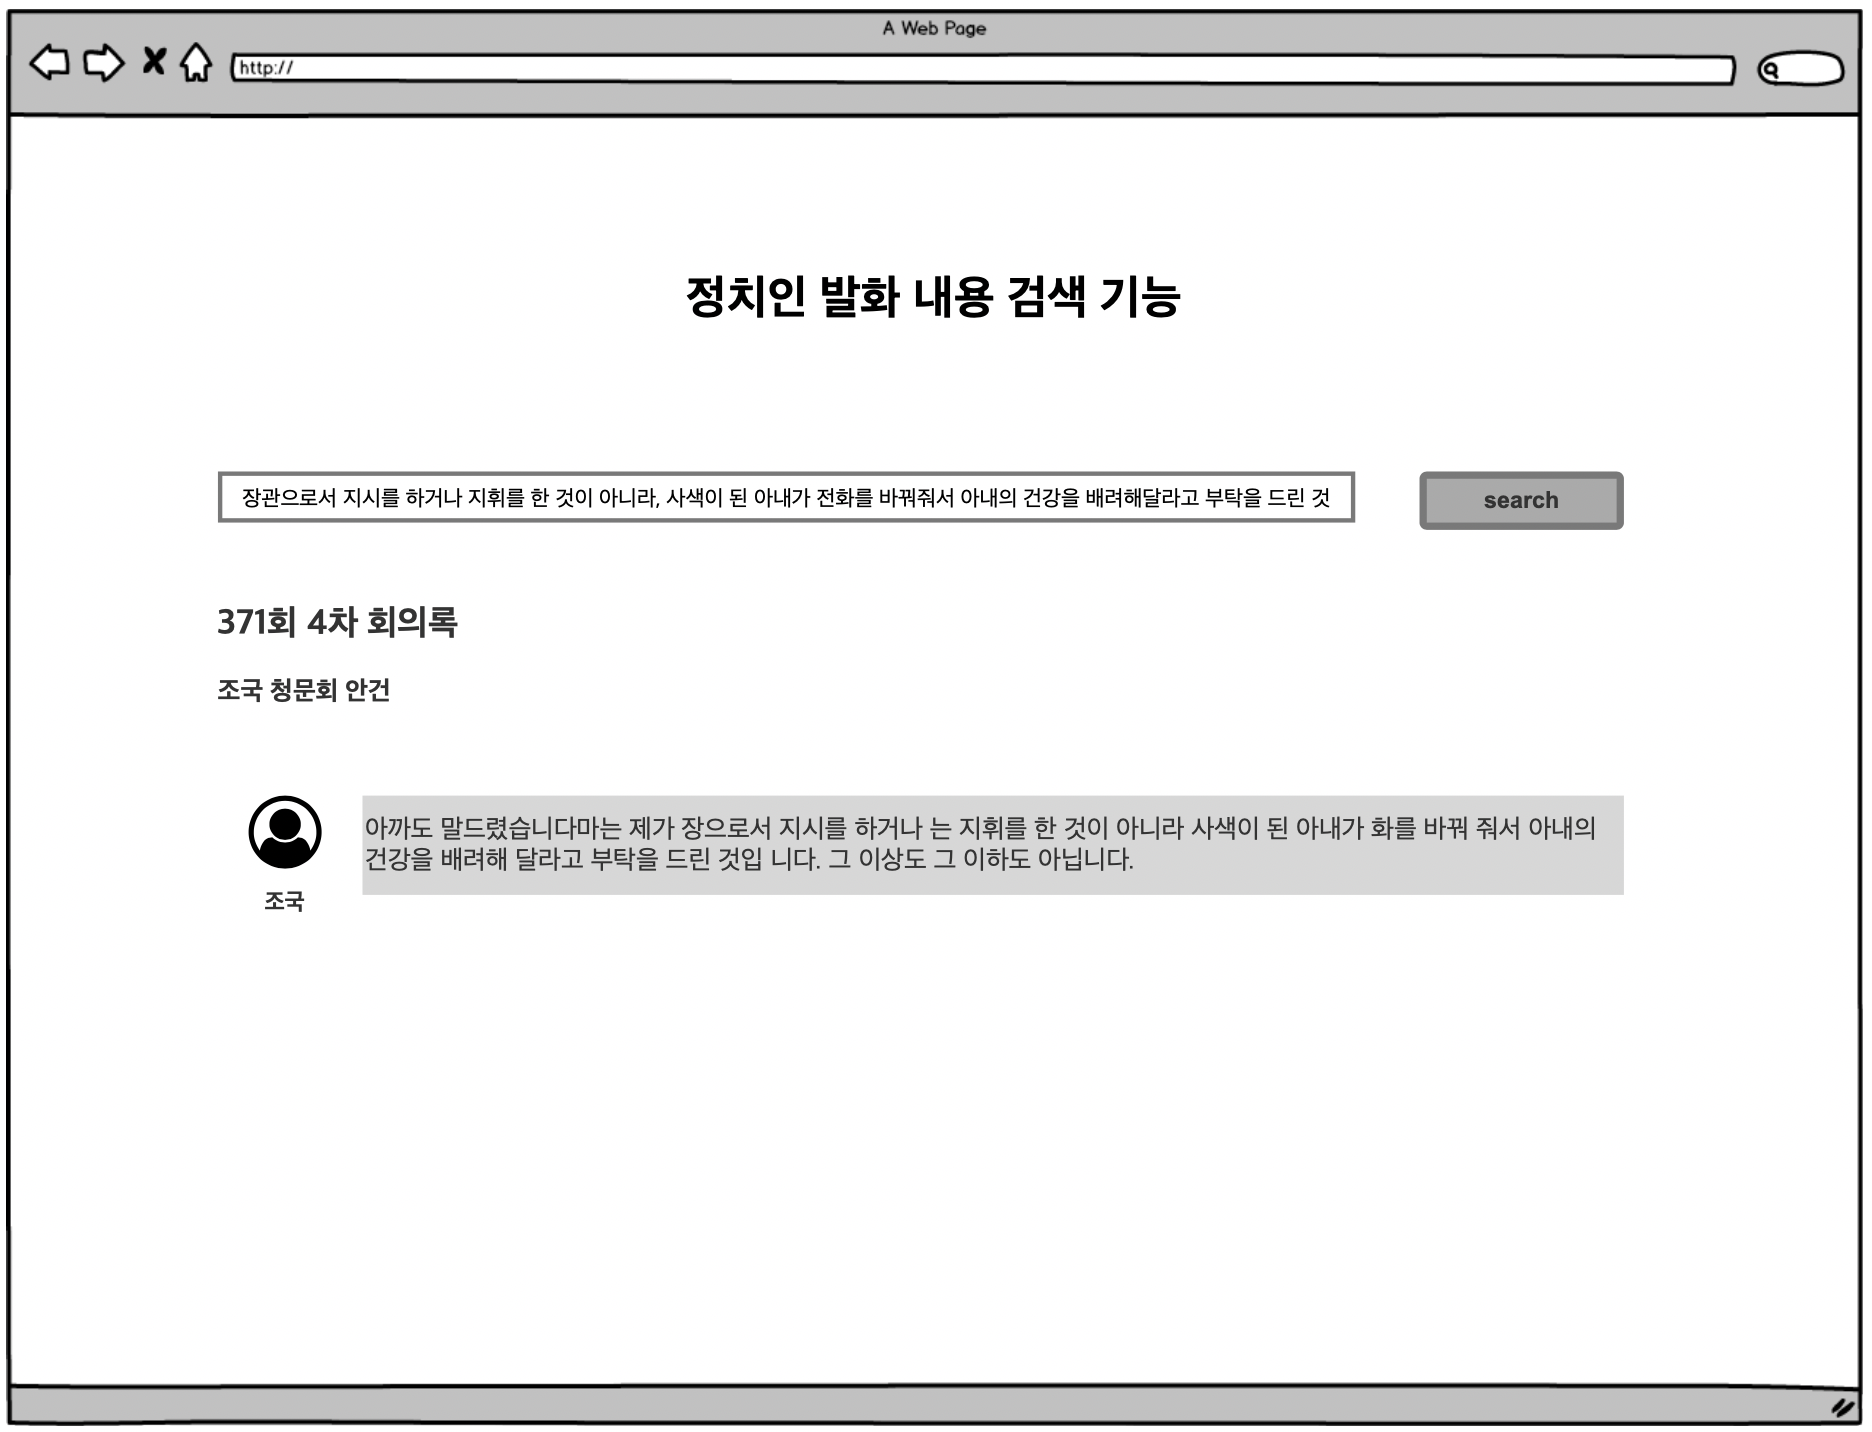
\includegraphics[width=89mm,scale=0.5]{fig/9.png}}
	\caption{Searching real speech of the politician function}
	\label{fig}
	\end{figure}     
        \item \textit {Searching real speech of the politician function: }This page is useful if the user wants to judge article’s quotation is true or not. User can search the facts in the minutes data, by filling out the search bar. If the user copy quotation in the article and paste in the search bar, they can click the search button. If then, what the politician actually said is popped out below with name of the assembly minutes, and agenda when he said at.\\
        \end{enumerate}

    \vspace{30mm}
    \begin{enumerate}
    	\item \textit{Nugu service: }
	 \begin{enumerate}
    	\item \textit{Searching of the politicians function: } This function can search politician’s participated agendas. If the user utter curious politician, Nugu speaker send back most recent participated agenda of the politician.\\

        \item \textit{Looking up real speech of the politician in that agenda: } User can look up real speech of the politician. Nugu speaker speak out specific politician’s most recent utterance.\\
         \item \textit{Looking up real speech of the politician in that agenda: } User can request Nugu speaker to play back or forward speech of the politician. Nugu speaker speak out back and forward speech of current playing.\\
           \end{enumerate}
           
    \end{enumerate}
    
                \end{enumerate}


\end{document}

